% Raqeeb: final project documentation.
% Compile with XeLaTeX (Overleaf: Menu > Compiler > XeLaTeX) or Tectonic:  tectonic raqeeb_report.tex
% Figures are in figures/. IBM Plex Sans ships with TeX Live (the plex package); IBM Plex Sans
% Arabic does not, so its files are in fonts/ (SIL Open Font License, fonts/OFL.txt).

\newcommand{\groupnumber}{2}   % leave empty to omit the line from the title page

\documentclass[11pt,a4paper]{article}

\usepackage[margin=2.3cm,headheight=14pt]{geometry}
\usepackage{fontspec}
\usepackage{xcolor}
\usepackage{graphicx}
\usepackage{booktabs}
\usepackage{tabularx}
\usepackage{array}
\usepackage{multirow}
\usepackage{enumitem}
\usepackage{caption}
\usepackage{subcaption}
\usepackage{float}
\usepackage{fancyhdr}
\usepackage[nobottomtitles*]{titlesec}
\renewcommand{\bottomtitlespace}{0.12\textheight}
\usepackage{tikz}
\usetikzlibrary{arrows.meta,positioning,fit,backgrounds}
\usepackage[hidelinks]{hyperref}

\setmainfont{IBMPlexSans}[Extension=.otf,UprightFont=*-Regular,BoldFont=*-Bold,ItalicFont=*-Italic,BoldItalicFont=*-BoldItalic]
\setmonofont{IBMPlexMono}[Extension=.otf,UprightFont=*-Regular,BoldFont=*-Bold]
% Headings use SemiBold. The sans family must also differ from the main one in some setting: declared
% identically, fontspec shares one family between the two and polyglossia's switch to Arabic fails.
\setsansfont{IBMPlexSans}[Extension=.otf,UprightFont=*-Regular,BoldFont=*-SemiBold,ItalicFont=*-Italic,BoldItalicFont=*-SemiBoldItalic]

% polyglossia (and the bidi package it loads) must come after hyperref, tikz and graphicx
\usepackage{polyglossia}
\setdefaultlanguage{english}
\setotherlanguage{arabic}
\newfontfamily\arabicfont[Script=Arabic,Path=fonts/,Extension=.ttf,UprightFont=*-Regular,BoldFont=*-Bold]{IBMPlexSansArabic}

\definecolor{navy}{HTML}{0D2A61}
\definecolor{soft}{HTML}{EEF2FA}
\definecolor{muted}{HTML}{5A6475}
\hypersetup{colorlinks=true,linkcolor=navy,urlcolor=navy,citecolor=navy}

\titleformat{\section}{\sffamily\Large\bfseries\color{navy}}{\thesection}{0.6em}{}
\titleformat{\subsection}{\sffamily\large\bfseries\color{navy}}{\thesubsection}{0.6em}{}
\titleformat{\subsubsection}{\sffamily\normalsize\bfseries}{}{0em}{}
\titlespacing*{\section}{0pt}{1.6em}{0.7em}
\titlespacing*{\subsection}{0pt}{1.2em}{0.5em}

\captionsetup{font=small,labelfont={bf,color=navy},format=plain,margin=0.5cm}
\setlist{itemsep=0.25em,topsep=0.4em}
\setlength{\parskip}{0.45em}
\setlength{\parindent}{0pt}
\setlength{\emergencystretch}{3em}
\brokenpenalty=10000
\renewcommand{\arraystretch}{1.2}

\pagestyle{fancy}
\fancyhf{}
\fancyhead[L]{\sffamily\small\color{muted}Raqeeb: final project documentation}
\fancyhead[R]{\sffamily\small\color{muted}\thepage}
\renewcommand{\headrulewidth}{0.4pt}

\newcommand{\ar}[1]{\textarabic{#1}}
\newcommand{\code}[1]{\texttt{#1}}
\newcolumntype{L}{>{\raggedright\arraybackslash}X}
\newcolumntype{P}[1]{>{\raggedright\arraybackslash}p{#1}}
\newcolumntype{B}[1]{>{\raggedright\arraybackslash\bfseries}p{#1}}

\begin{document}

% ------------------------------------------------------------------ title page
\begin{titlepage}
\centering
\vspace*{1.2cm}

\includegraphics[width=2.8cm]{figures/logo.png}\par
\vspace{0.8cm}
{\sffamily\fontsize{38}{44}\selectfont\bfseries\color{navy} Raqeeb\par}
\vspace{0.2cm}
{\fontsize{30}{36}\selectfont\color{navy}\ar{رقيب}\par}
\vspace{0.8cm}
{\Large Detecting prohibited items in X-ray baggage scans,\\ and reporting them to the right authority by voice\par}
\vspace{1.2cm}
{\large\sffamily Final project documentation\par}
{\large AI Model Development Bootcamp\par}
{\large\ar{معسكر بناء وتطوير نماذج الذكاء الاصطناعي}\par}
\if\relax\detokenize\expandafter{\groupnumber}\relax\else
  \vspace{0.3cm}{\large Group \groupnumber\par}
\fi
\vspace{1.4cm}
\begin{tabular}{rl}
Khalid Al Dosari & \ar{خالد آل دوسري} \\
Nawaf Alsharani & \ar{نواف الشهراني} \\
Yazeed Bin Shihah & \ar{يزيد بن شيحة} \\
Omar Al-Dhawyan & \ar{عمر الضويان} \\
\end{tabular}\par
\vfill
{\small
Code: \url{https://github.com/khaliddosari/Raqeeb}\\
Live demo: \url{https://raqeeb.khalid-ai.dev}\par}
\vspace{0.4cm}
{\small\color{muted} September 2026\par}
\end{titlepage}

{\setlength{\parskip}{0pt}\tableofcontents}
\newpage

% ------------------------------------------------------------------ 1
\section{Project information}

\subsection{Name and team}

\textbf{Raqeeb} (\ar{رقيب}, Arabic for ``watcher''). The team is Khalid Al Dosari, Nawaf Alsharani,
Yazeed Bin Shihah and Omar Al-Dhawyan; section~\ref{sec:team} lists who did what.

\subsection{The idea in brief}

Raqeeb helps the officers who screen bags at a security checkpoint. A detector trained on X-ray
scans marks five kinds of prohibited item: guns, knives, pliers, scissors and wrenches. When the
officer checks the bag and confirms the find, Raqeeb takes over the paperwork and the phone: it
writes the incident report in Arabic, works out which authority should respond, sends them the
report, and calls them to request a team, holding the conversation itself in Saudi Arabic.

\subsection{The problem}

Screening at airports and at the secure entrances of large events depends on an operator reading
each X-ray image in a few seconds while a queue waits. Two parts of the job are slow and easy to
get wrong:

\begin{itemize}
  \item \textbf{Finding the item.} Prohibited items are often small, thin, rotated, or buried under
        electronics and clothing, and X-ray images show everything in the bag on top of everything
        else.
  \item \textbf{Everything after finding it.} The officer has to keep the passenger and the bag in
        place, write an incident report, decide whether it is a police matter or an airport security
        matter, and phone that authority. While this happens the lane is stopped, and until the call
        is made nobody is on the way.
\end{itemize}

\subsection{Target users}

\begin{itemize}
  \item \textbf{Screening officers} at checkpoints: airport and private aviation terminals and the
        entrances of major events. They run the detector, confirm or reject each find, and scan the
        bag carrier's pass.
  \item \textbf{Security supervisors}, who follow each incident on the dashboard from detection to
        dispatch.
  \item \textbf{Responding authorities}: the police for guns and knives, airport security for tools.
        They receive a structured report and a phone call.
  \item \textbf{Buyers}: government and private security agencies that run checkpoints.
\end{itemize}

\subsection{Value}

\begin{itemize}
  \item \textbf{A second pair of eyes on every scan.} The detector marks the item and states how
        confident it is.
  \item \textbf{Minutes saved after a find.} Once the officer confirms, the report, the choice of
        authority and the call happen without further work from the officer.
  \item \textbf{Consistent reports.} Every report has the same structure, in formal Arabic, and its
        key facts are copied from the detection rather than retyped.
  \item \textbf{A person stays in control.} Nothing is reported until an officer has checked the bag
        by hand.
\end{itemize}

% ------------------------------------------------------------------ 2
\section{How the solution works}
\label{sec:flow}

\subsection{Input, processing and output}

\textbf{What the user puts in}
\begin{enumerate}
  \item An X-ray image of a bag: an uploaded image, or a frame from the scanner's video.
  \item A decision: after checking the bag by hand, the officer confirms the detection or rejects it
        as a false alarm.
  \item The bag carrier's details, by scanning the QR code on their boarding pass or event badge,
        or by typing their name and ID number.
\end{enumerate}

\textbf{What happens inside the system}
\begin{enumerate}
  \item The detector (YOLOv8s-OBB) finds prohibited items and returns each one's class, confidence
        and oriented box. On video, a tracker keeps one ID per physical item as it moves along the
        belt.
  \item The incident waits for the officer's decision. A rejection closes it as a false alarm.
  \item A workflow (LangGraph) builds the incident record from the detection, the verification, the
        carrier's details and the checkpoint.
  \item A language model (gpt-4o-mini) assigns a severity and a recommended action, returned as
        JSON, and writes the narrative report in Arabic.
  \item A routing table maps the item to the responsible authority: guns and knives to the police;
        pliers, scissors and wrenches to airport security.
  \item The report is sent to that authority, and a voice agent (gpt-realtime) calls them: it
        briefs them in Saudi Arabic, answers their questions, and records whether they are sending
        a team.
\end{enumerate}

\textbf{What the user gets back}
\begin{itemize}
  \item The annotated image, with the item, its class and confidence, and the authority it routes to.
  \item The incident report: a structured record, the Arabic narrative, and the checkpoint's
        situation.
  \item A live transcript of the call, the authority's decision, and a ``judgment'' panel that shows
        why the system acted as it did.
\end{itemize}

\begin{figure}[H]
\centering
\begin{tikzpicture}[
  font=\sffamily\footnotesize,
  execute at begin node={\hyphenpenalty=10000},
  box/.style={draw=navy,rounded corners=3pt,fill=white,align=center,minimum height=1.35cm,text width=2.75cm,inner sep=3pt},
  human/.style={box,fill=soft,dashed},
  arr/.style={-{Stealth[length=2.2mm]},thick,navy},
  lane/.style={draw=none,fill=navy!6,rounded corners=6pt}]
  \node[box] (img) {X-ray image\\or video frame};
  \node[box,right=0.55cm of img] (det) {\textbf{YOLOv8s-OBB}\\class, confidence,\\box (+ tracking)};
  \node[human,right=0.55cm of det] (ver) {\textbf{Officer checks}\\the bag:\\confirm / reject};
  \node[box,right=0.55cm of ver] (rec) {Incident record\\+ carrier's pass\\(LangGraph)};
  \node[box,below=1.05cm of rec] (llm) {\textbf{gpt-4o-mini}\\severity (JSON)\\+ Arabic report};
  \node[box,left=0.55cm of llm] (route) {Routing table\\gun, knife: police\\tools: airport sec.};
  \node[box,left=0.55cm of route] (call) {\textbf{gpt-realtime}\\calls the authority\\in Saudi Arabic};
  \node[box,left=0.55cm of call] (out) {Dispatch decision\\+ transcript\\on the dashboard};
  \draw[arr] (img) -- (det);
  \draw[arr] (det) -- (ver);
  \draw[arr] (ver) -- (rec);
  \draw[arr] (rec) -- (llm);
  \draw[arr] (llm) -- (route);
  \draw[arr] (route) -- (call);
  \draw[arr] (call) -- (out);
  \node[font=\sffamily\scriptsize\color{muted},above=0.05cm of img] {INPUT};
  \node[font=\sffamily\scriptsize\color{muted},above=0.05cm of det] {COMPUTER VISION};
  \node[font=\sffamily\scriptsize\color{muted},above=0.05cm of ver] {HUMAN IN THE LOOP};
  \node[font=\sffamily\scriptsize\color{muted},above=0.05cm of rec] {PROCESSING};
  \node[font=\sffamily\scriptsize\color{muted},below=0.05cm of llm] {LANGUAGE MODEL};
  \node[font=\sffamily\scriptsize\color{muted},below=0.05cm of call] {VOICE AGENT};
  \node[font=\sffamily\scriptsize\color{muted},below=0.05cm of out] {OUTPUT};
  \node[font=\sffamily\scriptsize\color{muted},below=0.05cm of route] {RULES};
  \begin{scope}[on background layer]
    \node[lane,fit=(img)(det)(ver)(rec),inner sep=0.45cm] {};
    \node[lane,fit=(out)(call)(route)(llm),inner sep=0.45cm] {};
  \end{scope}
\end{tikzpicture}
\caption{The flow of one incident. The dashed box is the only step a person performs; a rejection there
closes the incident. Everything after it runs without the officer.}
\label{fig:flow}
\end{figure}

\subsection{Two ways to hold the call}

The dispatch call happens in one of two places, and everything before it is identical:
\begin{itemize}
  \item \textbf{Signed in} (the team's demo), Raqeeb places a real phone call through Twilio, which
        bridges the audio straight to OpenAI's realtime model. The call audio never passes through
        our server.
  \item \textbf{A public visitor} to the live site plays the authority themselves: the same Arabic
        conversation runs in their browser over WebRTC, and no phone call is placed. This keeps the
        public demo free of telephone costs and unable to ring anyone.
\end{itemize}

% ------------------------------------------------------------------ 3
\section{Data}

\subsection{The X-ray dataset}

\begin{table}[H]
\centering
\small
\begin{tabularx}{\textwidth}{@{}B{3.1cm}L@{}}
\toprule
Name & Sixray, Roboflow project \code{sixray-gzyn7}, version 1 \\
Source & X-ray images from the SIXray security-inspection benchmark~\cite{sixray}, labelled with
         oriented boxes and exported from Roboflow on 1 September 2026 (CC BY 4.0) \\
Link & \url{https://universe.roboflow.com/khalid-abdullah-al-dosari/sixray-gzyn7} (download needs a
       Roboflow API key); original benchmark: \url{https://github.com/MeioJane/SIXray} \\
Type & Colour X-ray images of bags; each object labelled by class and an oriented bounding box
       (four corner points), in YOLOv8-OBB format \\
Size & 8,312 images with 15,668 labelled objects: 5,819 for training, 1,662 for validation and 831
       for testing \\
Target & The location and class of every prohibited item: Gun, Knife, Pliers, Scissors or Wrench \\
Images & Sizes vary widely (median 623 × 572 px, 7,689 distinct resolutions); letterboxed to 640 px
         for training \\
\bottomrule
\end{tabularx}
\caption{Dataset summary. All figures in this section come from \code{EDA.ipynb}.}
\end{table}

\begin{table}[H]
\centering
\small
\begin{tabular}{@{}lrrrr@{}}
\toprule
Class & Train & Validation & Test & Total \\
\midrule
Pliers   & 3,680 & 1,110 & 524 & 5,314 \\
Gun      & 3,024 &   888 & 474 & 4,386 \\
Wrench   & 1,943 &   530 & 306 & 2,779 \\
Knife    & 1,473 &   442 & 169 & 2,084 \\
Scissors &   779 &   206 & 120 & 1,105 \\
\midrule
All      & 10,899 & 3,176 & 1,593 & 15,668 \\
\bottomrule
\end{tabular}
\caption{Labelled objects per class. Pliers outnumber scissors 4.8 to 1.}
\label{tab:classes}
\end{table}

\subsection{Checks and preprocessing}

\begin{itemize}
  \item \textbf{Integrity.} Every image has a label file and every label file an image. No image is
        unreadable, no label line malformed, and no box degenerate or outside the image.
  \item \textbf{Duplicates and leakage.} A search for exact-duplicate images across all three splits
        found none, so no test image also appears in training.
  \item \textbf{Empty images.} 17 images contain no objects. They were kept: they show the model
        what a bag with nothing in it looks like.
  \item \textbf{Split balance.} Each class's share differs by at most 3.3 percentage points between
        splits, so the test set is representative.
  \item \textbf{Orientation.} Box angles cluster at 0° and 90°: on this dataset the
        labels are close to upright, which limits how much oriented boxes can help here.
  \item \textbf{Class imbalance.} Training images were oversampled by inverse class frequency: an
        image with scissors (weight 4.7) is listed several times per epoch, one with only pliers
        (weight 1.0) once. The training list grows from 5,819 to 10,701 entries, and the imbalance
        in what the model sees drops from 4.7 to 1.6.
  \item \textbf{Augmentation.} Ultralytics augments every image as it is loaded: mosaic, colour
        jitter, flips, rotation, translation, scale and shear. A duplicated image therefore looks
        different each time. For the final model, mosaic is switched off for the last 15 epochs so
        training ends on undistorted images.
\end{itemize}

\subsection{Video with ground truth, for tracking}

No public X-ray dataset contains video, so there was nothing to measure tracking against. The
script \code{make\_test\_video.py} therefore builds conveyor-belt footage from the 831 held-out test images and
carries their labels from frame to frame, so every object has a known identity. It adds the
behaviour that makes tracking hard: the belt stopping and reversing, speed changes, bags cut off at
the edge, overlapping bags, and changes in brightness and noise. Two clips (random seeds 7 and 21)
were generated. The dashboard's demo clip, \code{test\_clip.mp4} (25 seconds), has no ground truth
and is used only for display.

\subsection{Text inputs for the language model}

The language model is not trained on any data; it is given the incident record as JSON. Two
hand-written files feed that record: six checkpoint scenarios in Arabic (\code{agent/checkpoints.py}:
the event, the gate, the crowd, who carried the bag, what staff have done, and how responders should
arrive) and the routing table (\code{config/authority\_mapping.yaml}). The scenarios and every person in
the demo, including the names on the demo passes, are fictional.

% ------------------------------------------------------------------ 4
\section{The model and the technical solution}

\subsection{Problem types}

\begin{itemize}
  \item \textbf{Computer vision:} oriented object detection with five classes, plus multi-object
        tracking on video.
  \item \textbf{Large language model:} structured generation (a JSON severity and action) and
        report writing in Arabic, both through prompt engineering on a model reached by API.
  \item \textbf{Voice agent:} a realtime speech-to-speech model that holds a phone conversation and
        records the outcome through a function call.
\end{itemize}

No retrieval (RAG) is used, no Hugging Face model, and no language model is fine-tuned.

\subsection{Detection: YOLOv8-OBB}

\textbf{Why this model.}
\begin{itemize}
  \item The labels are oriented boxes, and YOLOv8-OBB~\cite{yolov8} predicts oriented boxes
        directly. In real scans items lie at any angle, and an upright box around a diagonal knife
        is mostly background.
  \item It is a one-stage detector that runs fast on a CPU: 58 ms per image for the final model at
        640 px on a desktop processor, which matters at a live screening lane.
  \item Ultralytics provides training, augmentation, evaluation and tracking in one tested library.
\end{itemize}

\textbf{Pretrained model and transfer learning.} Both models start from weights trained on DOTA~\cite{dota}, a
dataset of aerial images with oriented boxes. The whole network is then fine-tuned on the X-ray
data, with the output layer replaced for our five classes. The pretrained model on its own is
useless here, because DOTA's classes (planes, ships, swimming pools) have nothing to do with ours;
the baseline in table~\ref{tab:experiments} shows exactly that.

\begin{table}[H]
\centering
\small
\begin{tabularx}{\textwidth}{@{}B{2.6cm}LLL@{}}
\toprule
 & Baseline & Experiment 1 & Experiment 2 (final) \\
\midrule
Model & yolov8n-obb, DOTA weights, not trained on X-rays & yolov8n-obb, fine-tuned & yolov8s-obb, fine-tuned \\
Parameters & 3.1 M & 3.1 M & 11.4 M \\
Epochs & none & 50 (early-stop patience 15, never triggered) & 70 of 100: early stop, best at epoch 50 (patience 20) \\
Batch, image size & n/a, 640 & 163 (AutoBatch), 640 & 46 (AutoBatch), 640 \\
Data handling & none & oversampling, on-the-fly augmentation & the same, and no mosaic for the last 15 epochs \\
Hardware & CPU & NVIDIA A100 40 GB on Modal, 30.5 min, about US\$1 & A100 40 GB on Modal, about US\$3 to 4 \\
\bottomrule
\end{tabularx}
\caption{The three runs compared in section~\ref{sec:results}. Experiment 2 changes the model size, the epoch
budget and the end-of-training augmentation; everything else is the same.}
\label{tab:experiments}
\end{table}

\subsection{Tracking}

On video, Raqeeb runs Ultralytics' BoT-SORT tracker~\cite{botsort} with one change,
\path{trackers/raqeeb_botsort.yaml}: global motion compensation is switched off. It helps with a
handheld camera but hurts with a fixed scanner camera. A track counts as a threat only after it has
lasted two frames and reached a confidence of 0.5, so a single stray detection does not raise an
alarm. Video is analysed at 1280 px rather than the training size of 640; section~\ref{sec:tracking}
explains why.

\subsection{Language model: gpt-4o-mini}

The report step makes two calls to \code{gpt-4o-mini} through the OpenAI API
(\path{agent/providers/openai_llm.py}):

\begin{enumerate}
  \item \textbf{Severity and action}, answered only as JSON, with the action in Arabic:\\[0.2em]
        {\small\code{\{"severity": "low|medium|high|critical", "recommended\_action": "..."\}}}
  \item \textbf{The narrative report}, in formal Arabic, in five fixed sections: summary, detection and
        verification, people involved, risk assessment with reasons, and next steps.
\end{enumerate}

\textbf{How the vision result reaches the language model.} The detected class and confidence are
copied into the incident record exactly as the detector produced them, next to the officer's
verification, the carrier's details and the checkpoint's scenario. The model receives that whole
record as JSON and is told not to change the item, the confidence or the verification status. The
record sent to the authority and the phone call's briefing are both built from these structured
fields, not from the model's prose.

\textbf{Prompt engineering.} The team's first prototype (v1) asked the model, as a ``security
guard'', to write a report from six values placed in two sentences, and to leave nothing unfilled.
The production prompt (v2) passes the full record as JSON, names the facts that must not change, and
tells the model to state missing information plainly instead of inventing it. Both are compared in
\code{Report\_generation.ipynb}; section~\ref{sec:llm} has the results.

\subsection{Voice agent: gpt-realtime}

The call uses OpenAI's \code{gpt-realtime}, a speech-to-speech model. Its instructions are written in
Arabic (\code{agent/voice/authority\_prompts.py}): speak Saudi dialect, introduce itself as Raqeeb from
the checkpoint, give the item, the place, the suspect and the scenario, answer questions, and ask
whether a team will be sent. It has one tool, \code{record\_dispatch\_confirmation}, which records the
authority's answer. That tool is refused until the authority has actually spoken, because in an
early test the model recorded a ``confirmation'' after reaching voicemail.

\subsection{Application}

A LangGraph workflow (\code{agent/graph/workflow.py}) runs each incident. It pauses twice, for the
officer's verification and for the carrier's details, and resumes through HTTP requests; paused
incidents are stored in SQLite so that they survive the server restarting. The backend is FastAPI,
the dashboard is a React application, and every external service (language model, telephony) sits
behind an interface with a mock implementation, so the whole workflow runs in tests without keys.

% ------------------------------------------------------------------ 5
\section{Tools and technologies}

\begin{table}[H]
\centering
\small
\begin{tabularx}{\textwidth}{@{}P{4.2cm}L@{}}
\toprule
Tool & How it was used \\
\midrule
Python 3.12 & All backend, training, tracking and evaluation code \\
Jupyter notebooks & \code{EDA.ipynb} (data analysis and preprocessing), \code{Model\_Training.ipynb} (experiments and evaluation), \code{Report\_generation.ipynb} (prompt comparison) \\
Roboflow & Hosting the labelled dataset and exporting it in YOLOv8-OBB format \\
Ultralytics YOLOv8 (PyTorch) & Fine-tuning and running the detector; BoT-SORT tracking \\
Modal & A100 GPU training jobs (\code{modal\_train.py}) and hosting the backend (\code{modal\_app.py}) \\
OpenCV, NumPy, pandas, Matplotlib, seaborn, SciPy & Image handling, data analysis, charts, and the tracking metrics (optimal matching with SciPy) \\
OpenAI API & \code{gpt-4o-mini} for the severity JSON and the Arabic report; \code{gpt-realtime} for the call \\
LangGraph & The incident workflow, its pauses for the officer, and its SQLite checkpoints \\
FastAPI, SQLAlchemy, SQLite & The REST and WebSocket backend and the incident store \\
Twilio & Outbound phone calls, bridged to OpenAI's SIP endpoint \\
React, Vite, TypeScript, Tailwind, shadcn/ui & The dashboard, in English and Arabic (right to left) \\
Vercel, Cloudflare & Hosting the dashboard; the \code{raqeeb.khalid-ai.dev} domain \\
GitHub & Version control and collaboration, including pull requests between branches \\
uv & Locked, reproducible Python dependencies (\code{uv.lock}); \code{requirements.txt} pins the same versions \\
pytest & 40 automated tests that drive the workflow with mock providers \\
Playwright & Rendering the demo passes and share images; taking the screenshots in this report \\
Claude Code & AI coding assistant, used for implementation, debugging, code review and documentation \\
\bottomrule
\end{tabularx}
\caption{Tools and what each was used for.}
\end{table}

% ------------------------------------------------------------------ 6
\section{Interfaces}

All screenshots come from one complete run of the application on 18 September 2026: the bundled
test image, a demo pass for the private aviation terminal, and a call in which the ``police'' side
was a recorded Arabic reply. The dashboard has five numbered panels that follow the incident from
left to right and top to bottom.

\begin{figure}[H]
\centering
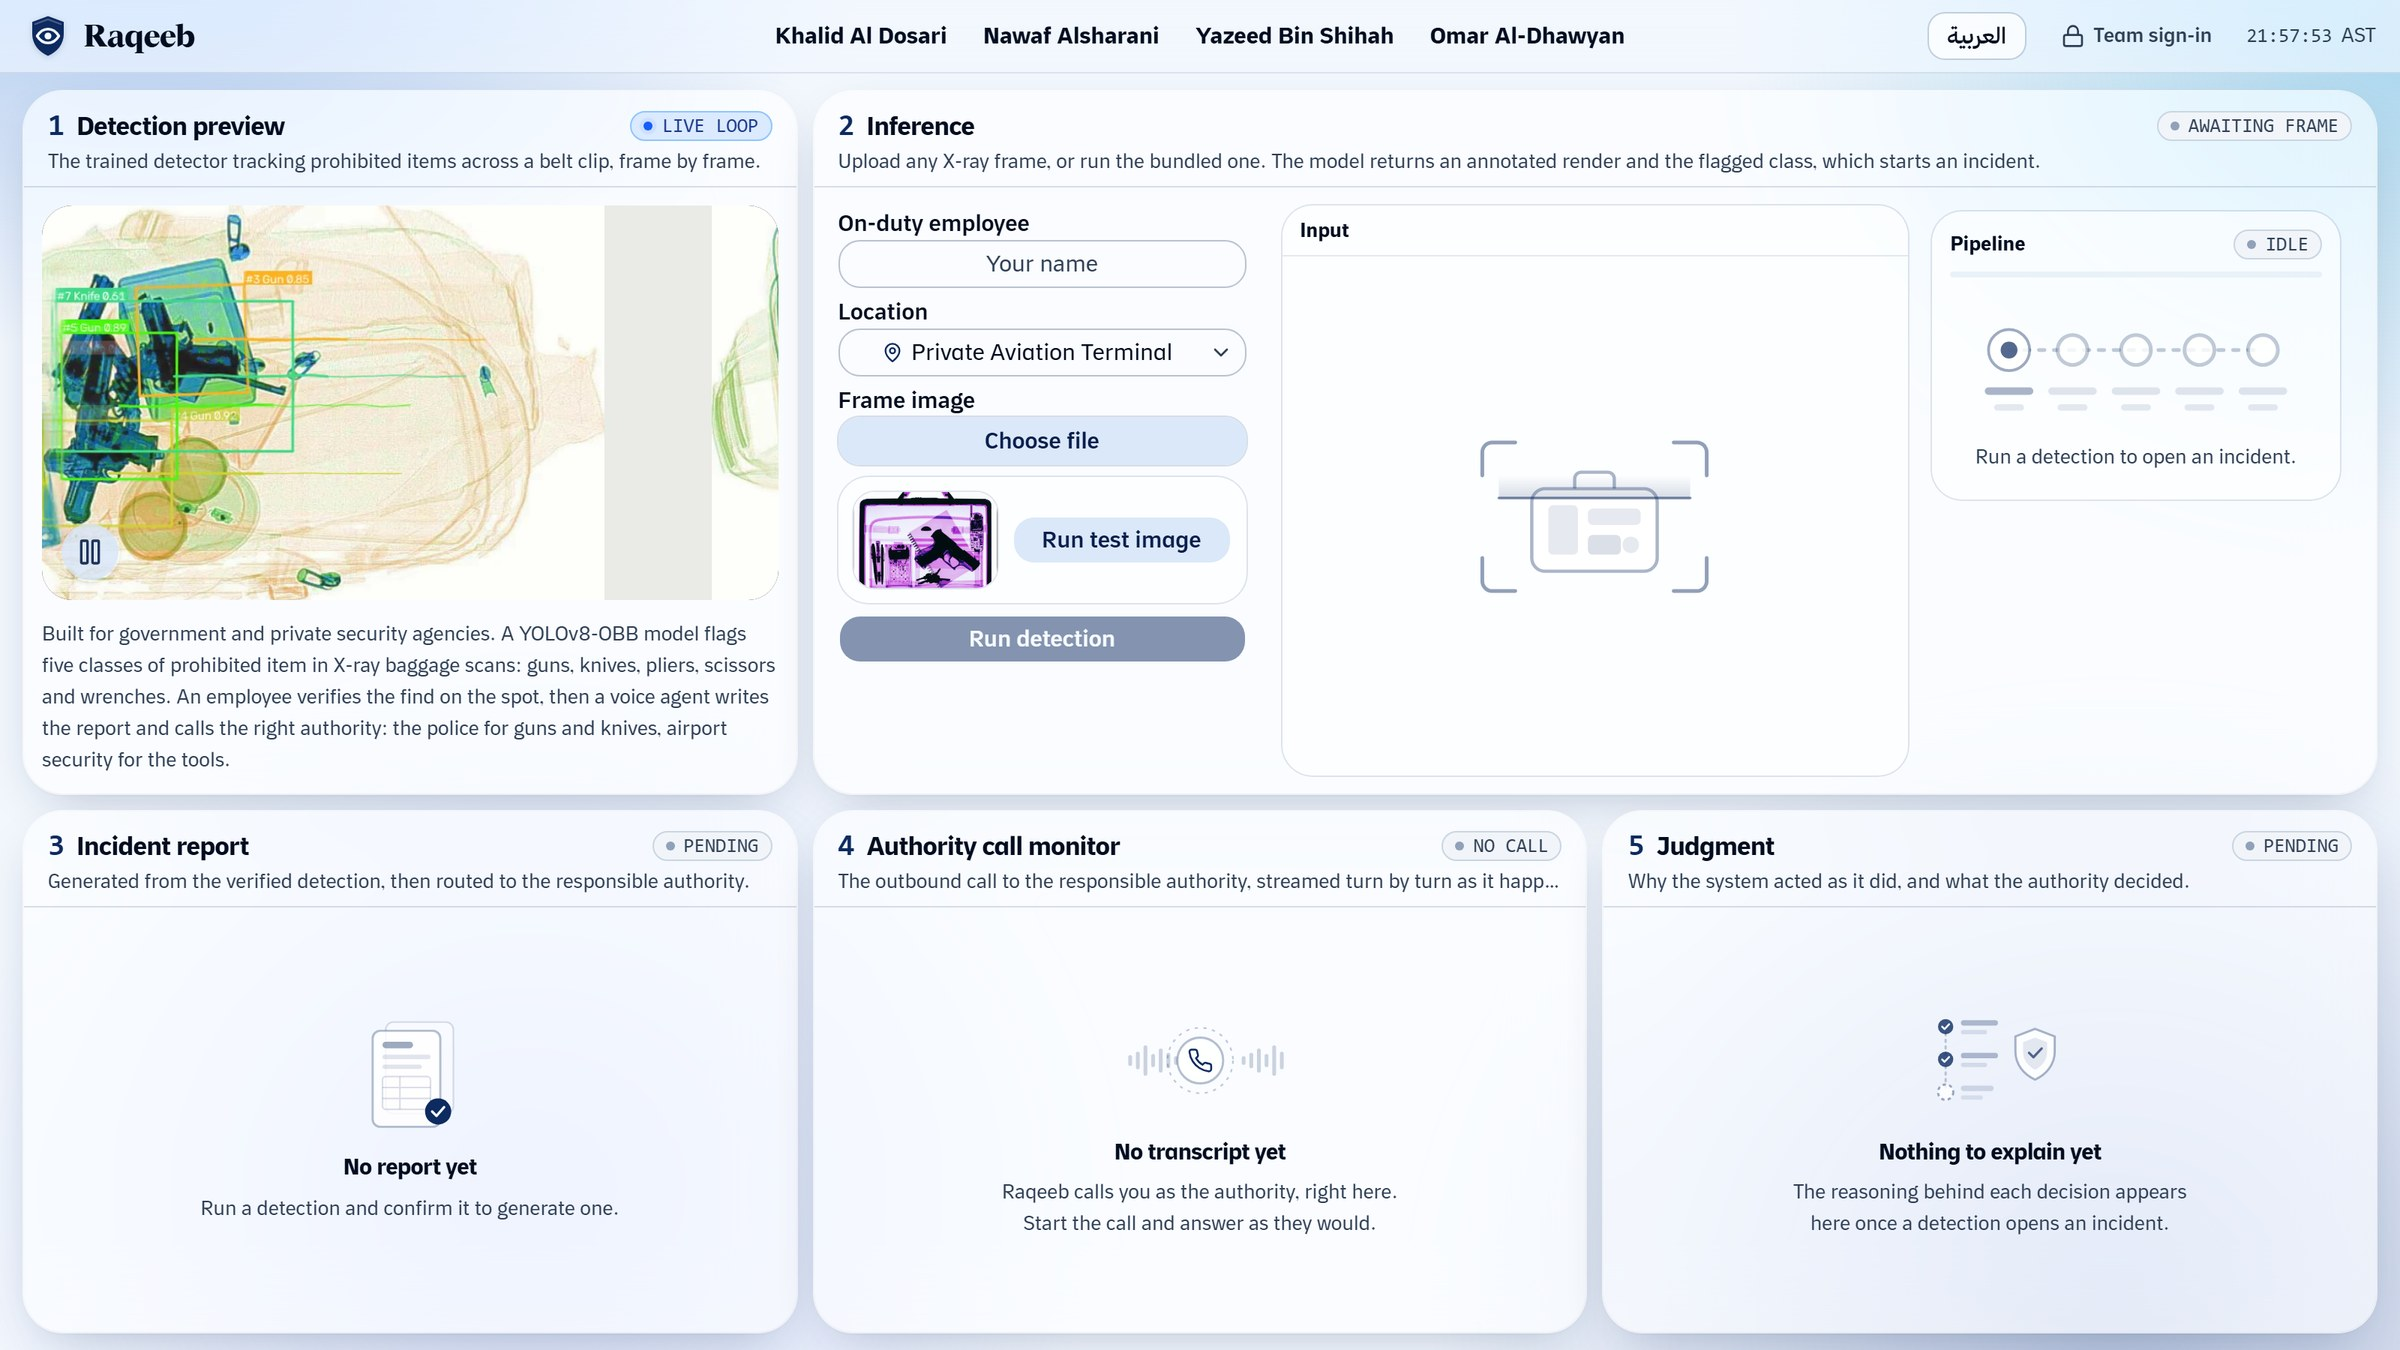
\includegraphics[width=\textwidth]{figures/ui_home.jpg}
\caption{\textbf{Home page}, before a run. Panel~1 plays the tracker on a belt clip; panel~2 is where
the officer enters their name and checkpoint and runs a detection; panels 3 to 5 (report, call,
judgment) wait for an incident. The header carries the team, the language switch and the local time.}
\end{figure}

\begin{figure}[H]
\centering
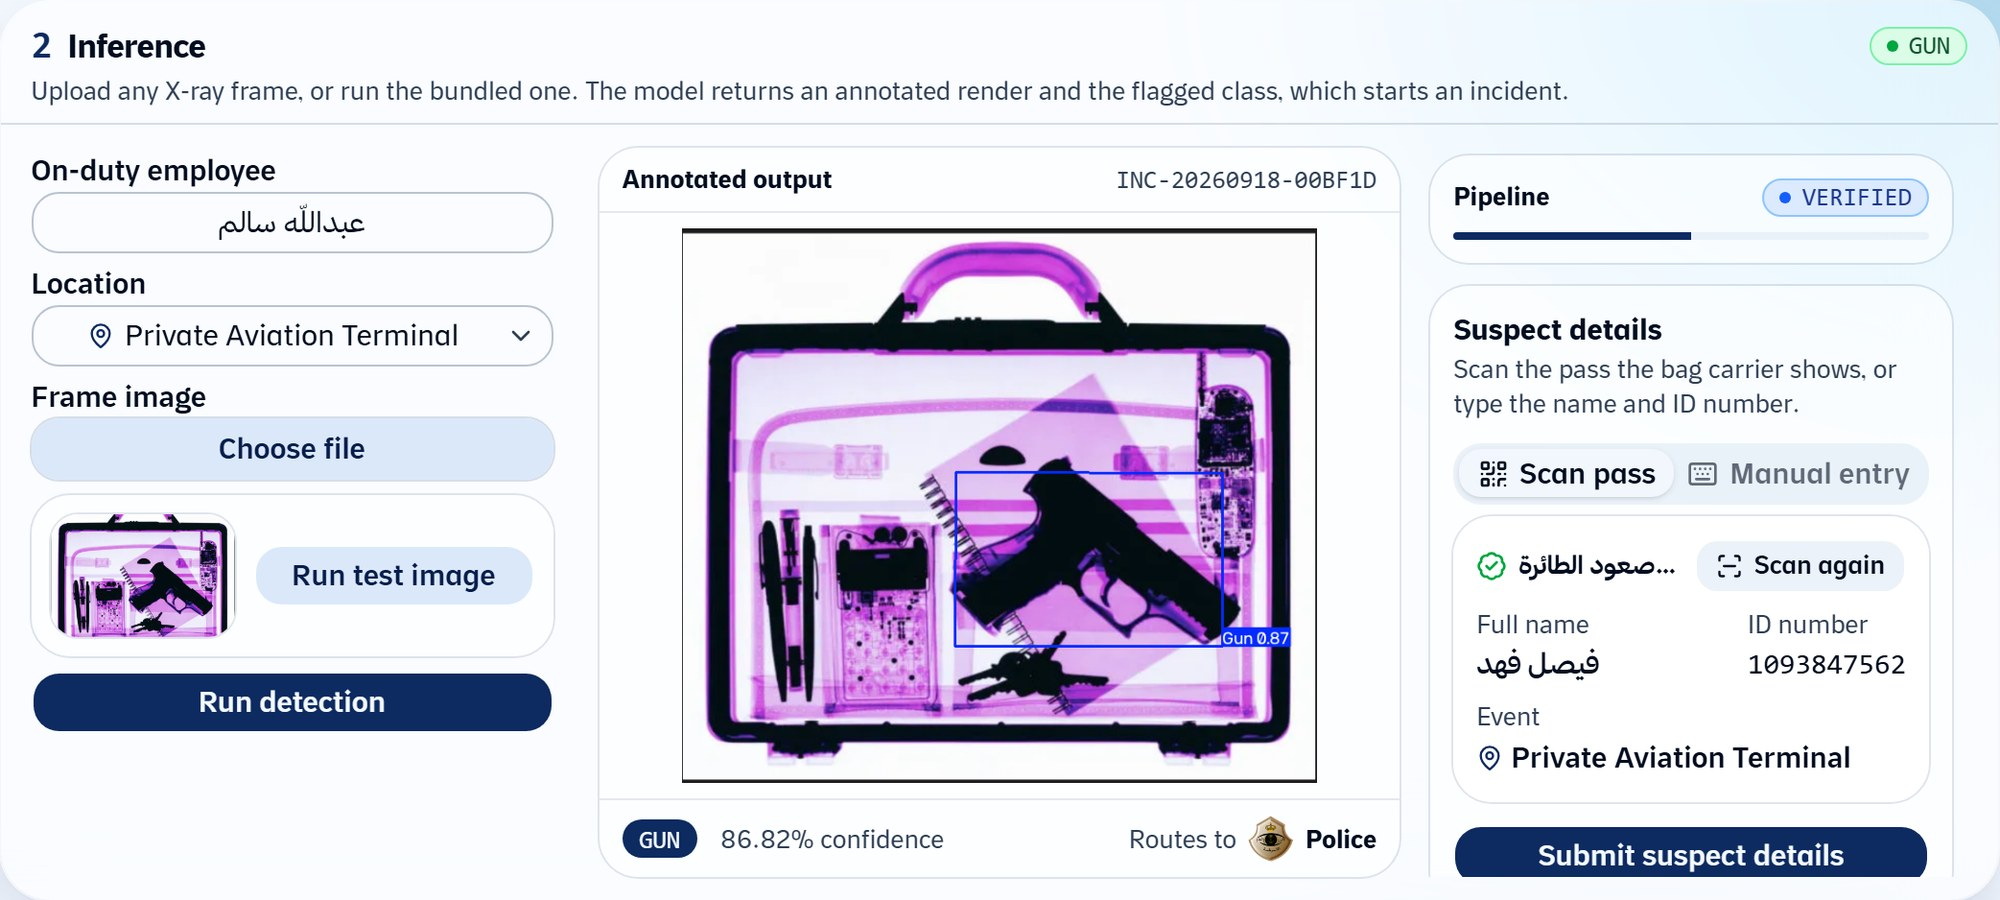
\includegraphics[width=\textwidth]{figures/ui_input_suspect.jpg}
\caption{\textbf{Input and first result.} The inference panel after a detection has been confirmed:
the annotated image (a gun, 86.82\% confidence), the authority it routes to (police), the pipeline
status, and the next input, the bag carrier's details, filled here by scanning a demo pass. The
officer can type the details instead under ``Manual entry''.}
\end{figure}

\begin{figure}[H]
\centering
\begin{subfigure}[t]{0.49\textwidth}
  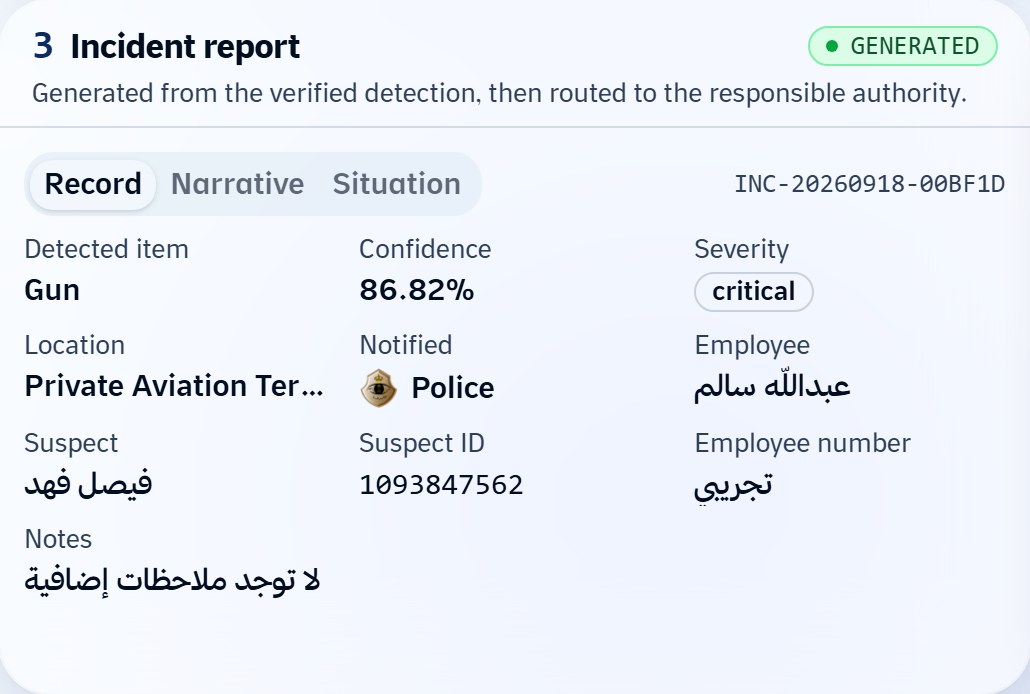
\includegraphics[width=\textwidth]{figures/ui_report_record.jpg}
  \caption{Record: the structured fields that are sent to the authority.}
\end{subfigure}\hfill
\begin{subfigure}[t]{0.49\textwidth}
  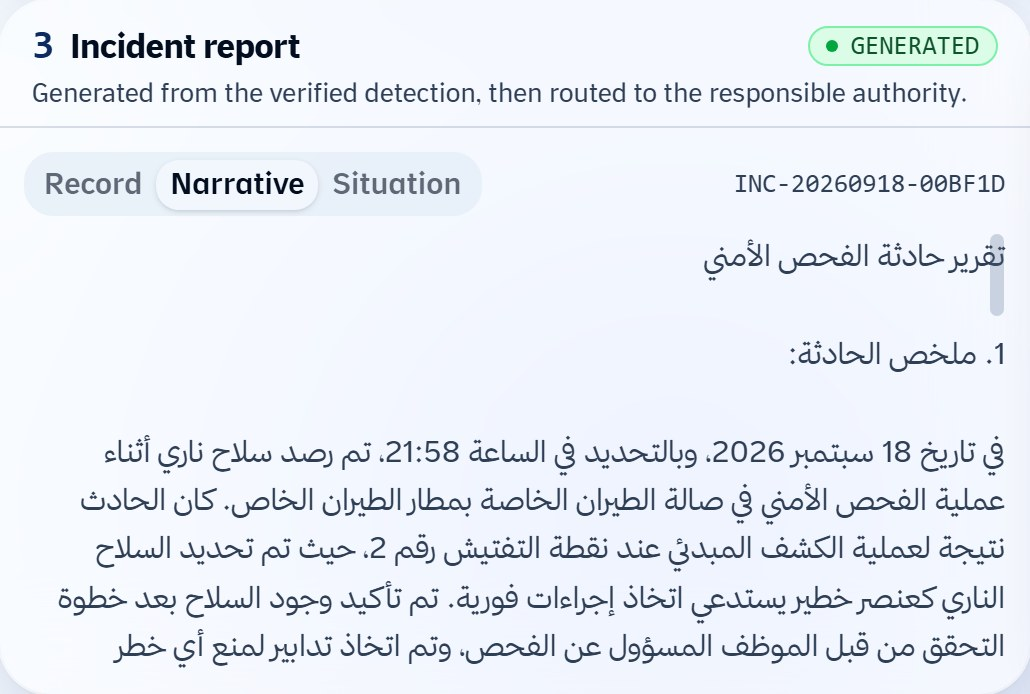
\includegraphics[width=\textwidth]{figures/ui_report_narrative.jpg}
  \caption{Narrative: the Arabic report written by gpt-4o-mini.}
\end{subfigure}
\caption{\textbf{Results: the incident report.} A third tab, ``Situation'', shows the checkpoint's
scenario that the report and the call draw on.}
\end{figure}

\begin{figure}[H]
\centering
\begin{subfigure}[t]{0.49\textwidth}
  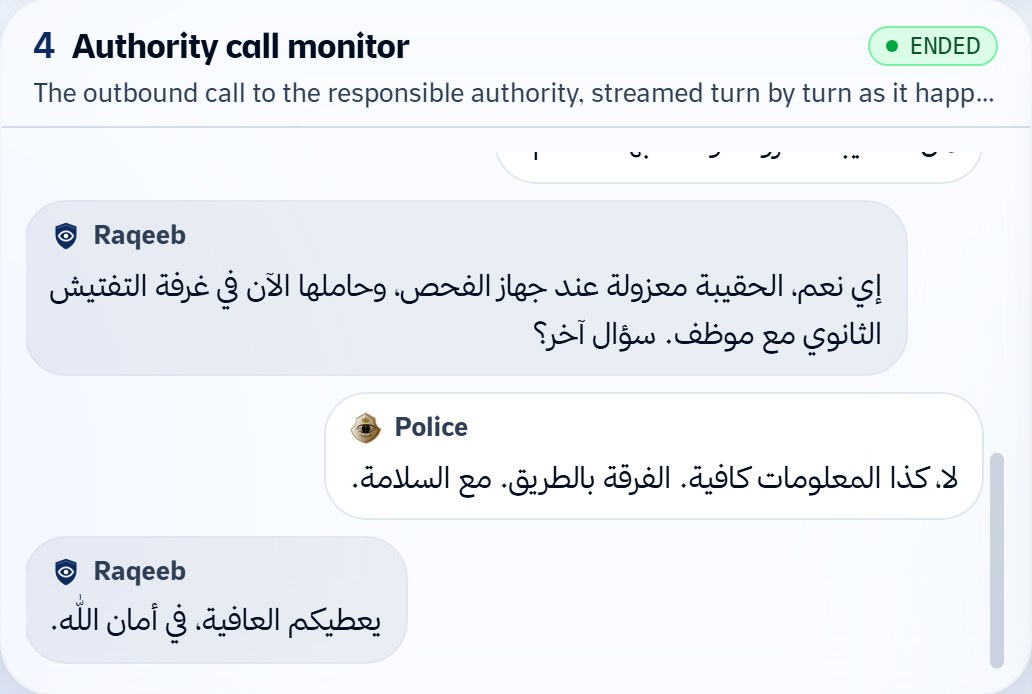
\includegraphics[width=\textwidth]{figures/ui_call.jpg}
  \caption{The call, streamed turn by turn as each side speaks.}
\end{subfigure}\hfill
\begin{subfigure}[t]{0.49\textwidth}
  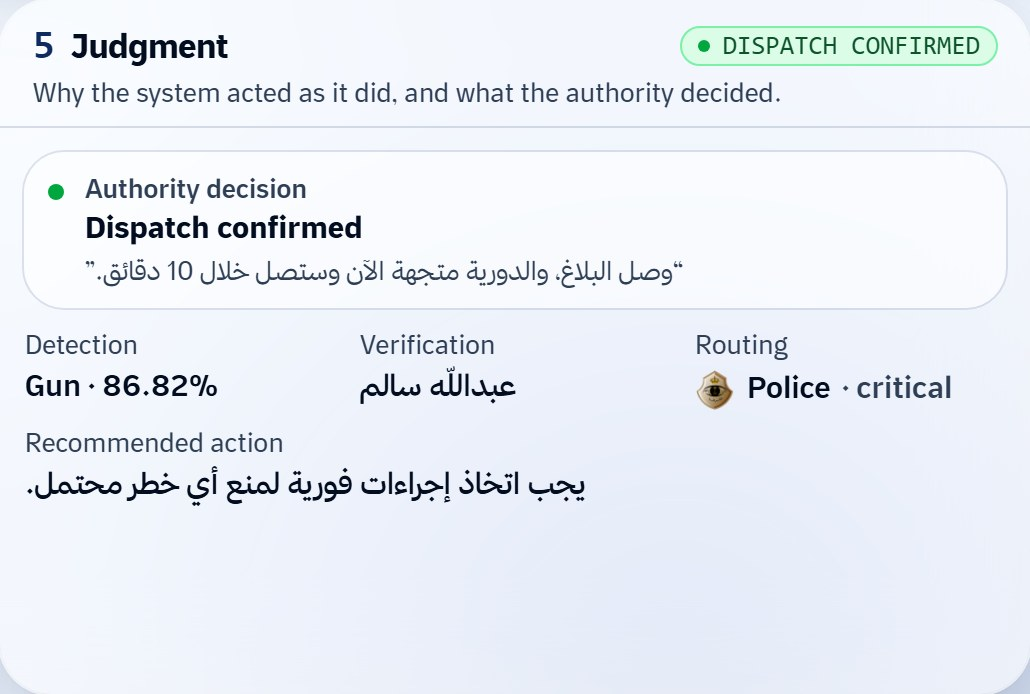
\includegraphics[width=\textwidth]{figures/ui_judgment.jpg}
  \caption{The judgment: the authority's decision and the reasons behind each step.}
\end{subfigure}
\caption{\textbf{The voice agent's conversation.} Raqeeb briefs the police in Saudi Arabic, answers,
and records the decision (``dispatch confirmed'') with the authority's own words.}
\end{figure}

\begin{figure}[H]
\centering
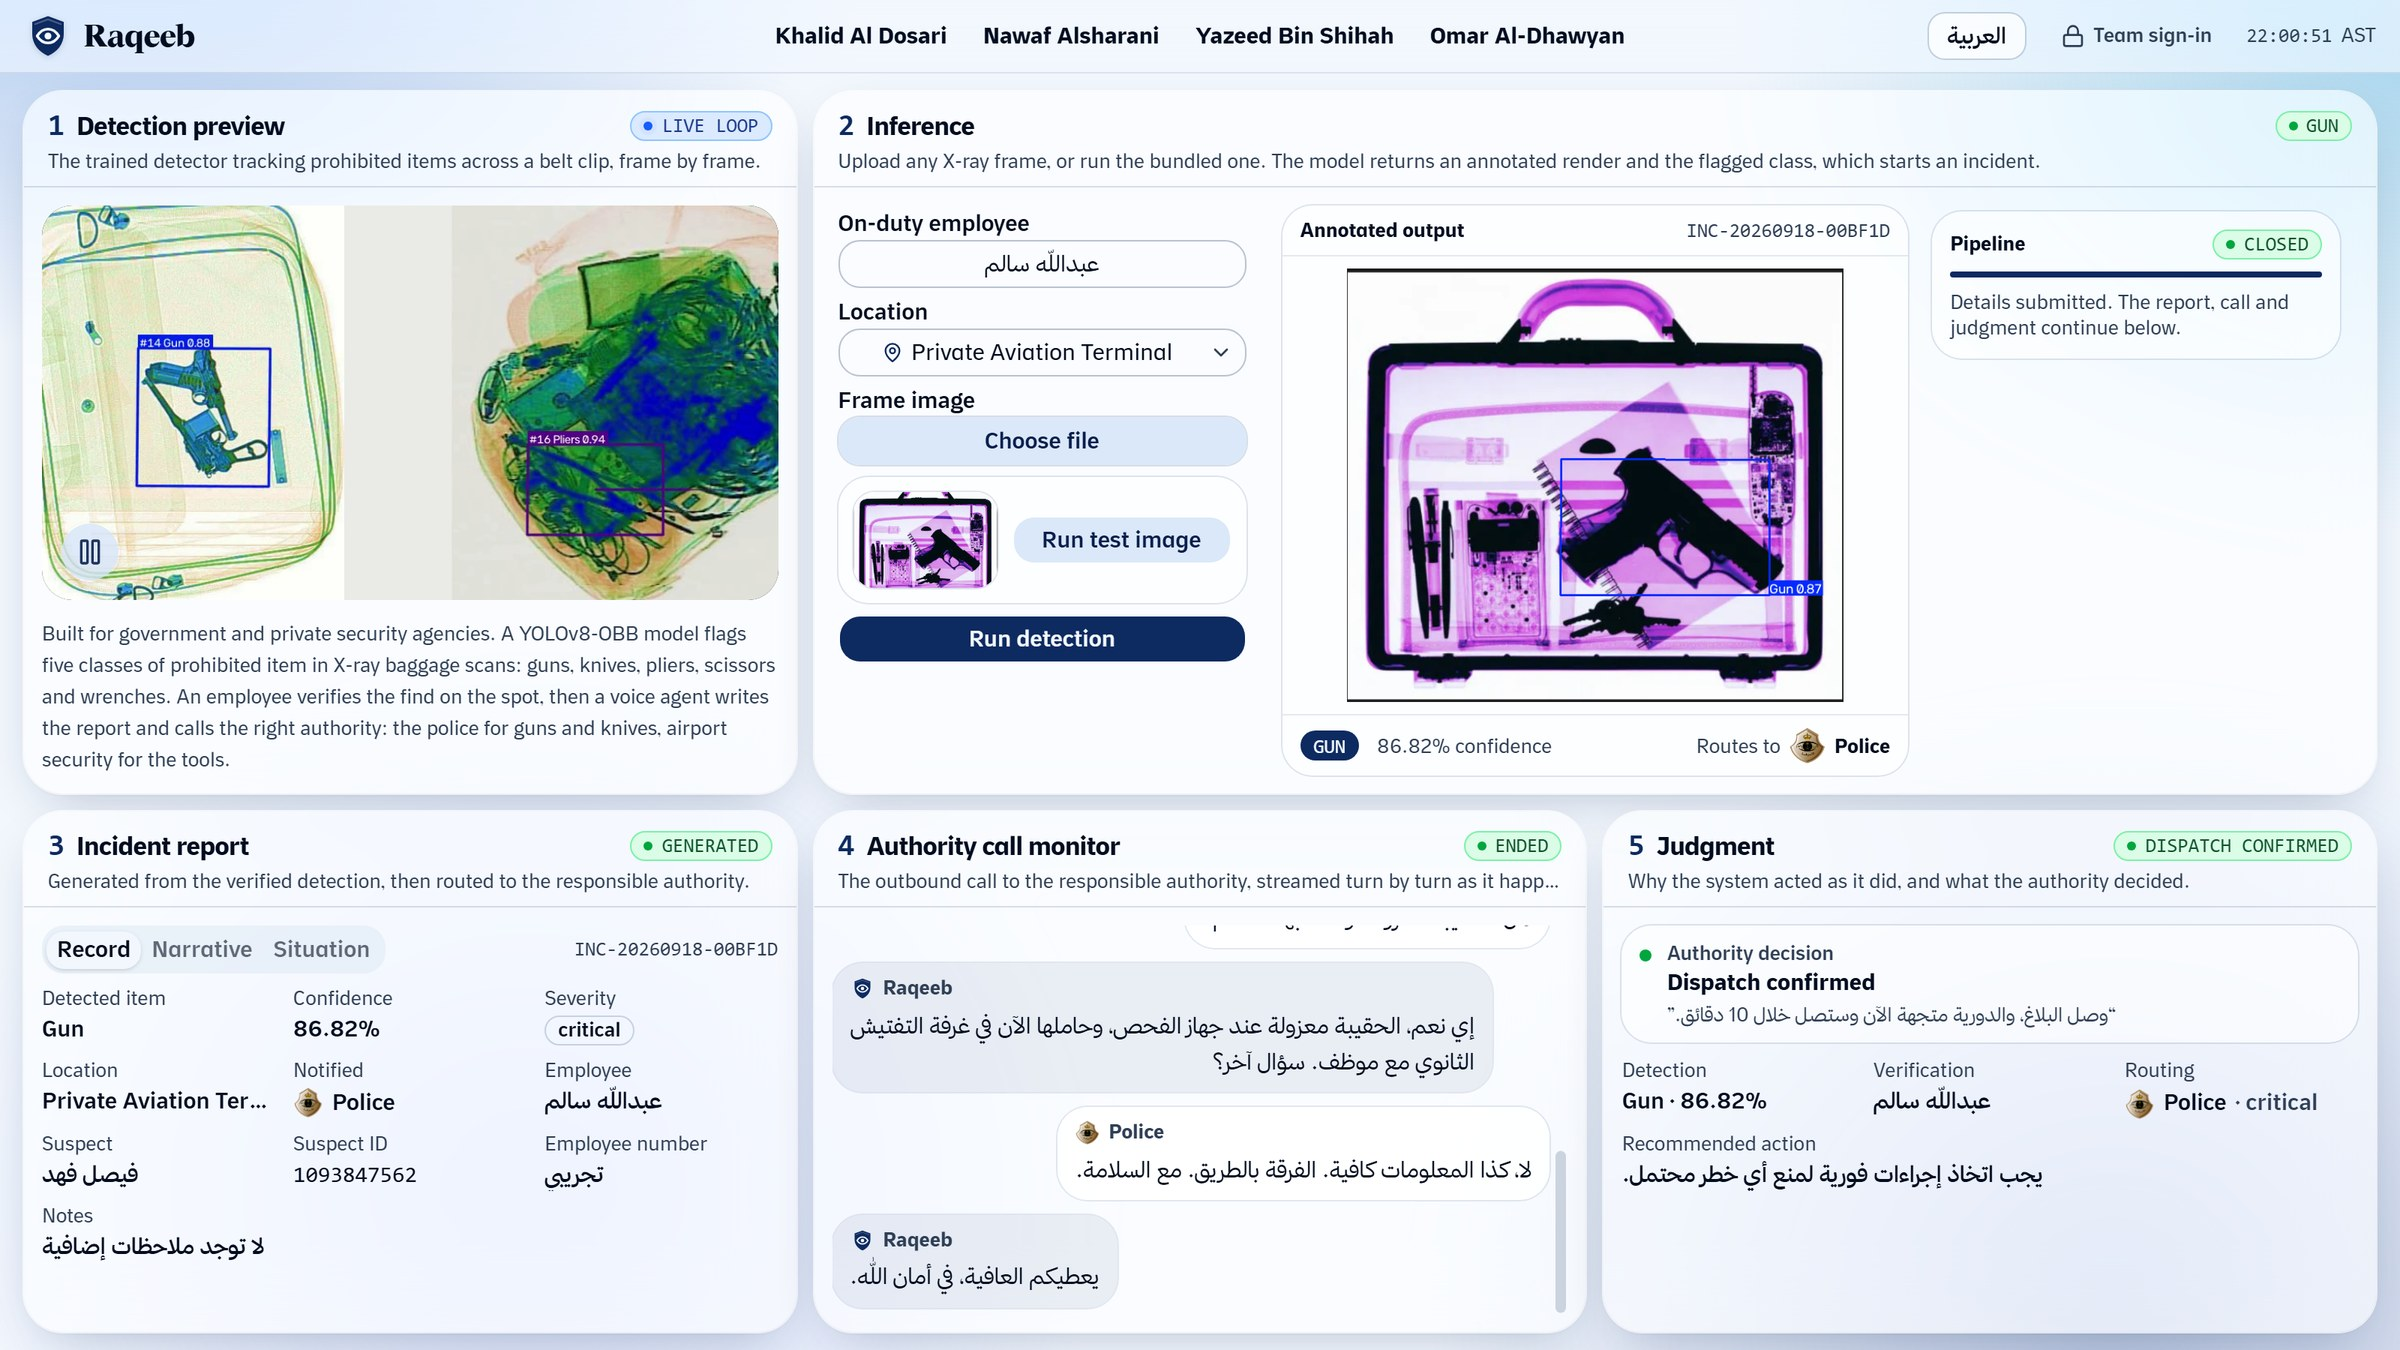
\includegraphics[width=\textwidth]{figures/ui_dashboard_closed.jpg}
\caption{\textbf{Dashboard: a completed incident.} All five panels after the call: detection,
report, transcript and judgment, with the pipeline status \textsc{closed}.}
\end{figure}

\begin{figure}[H]
\centering
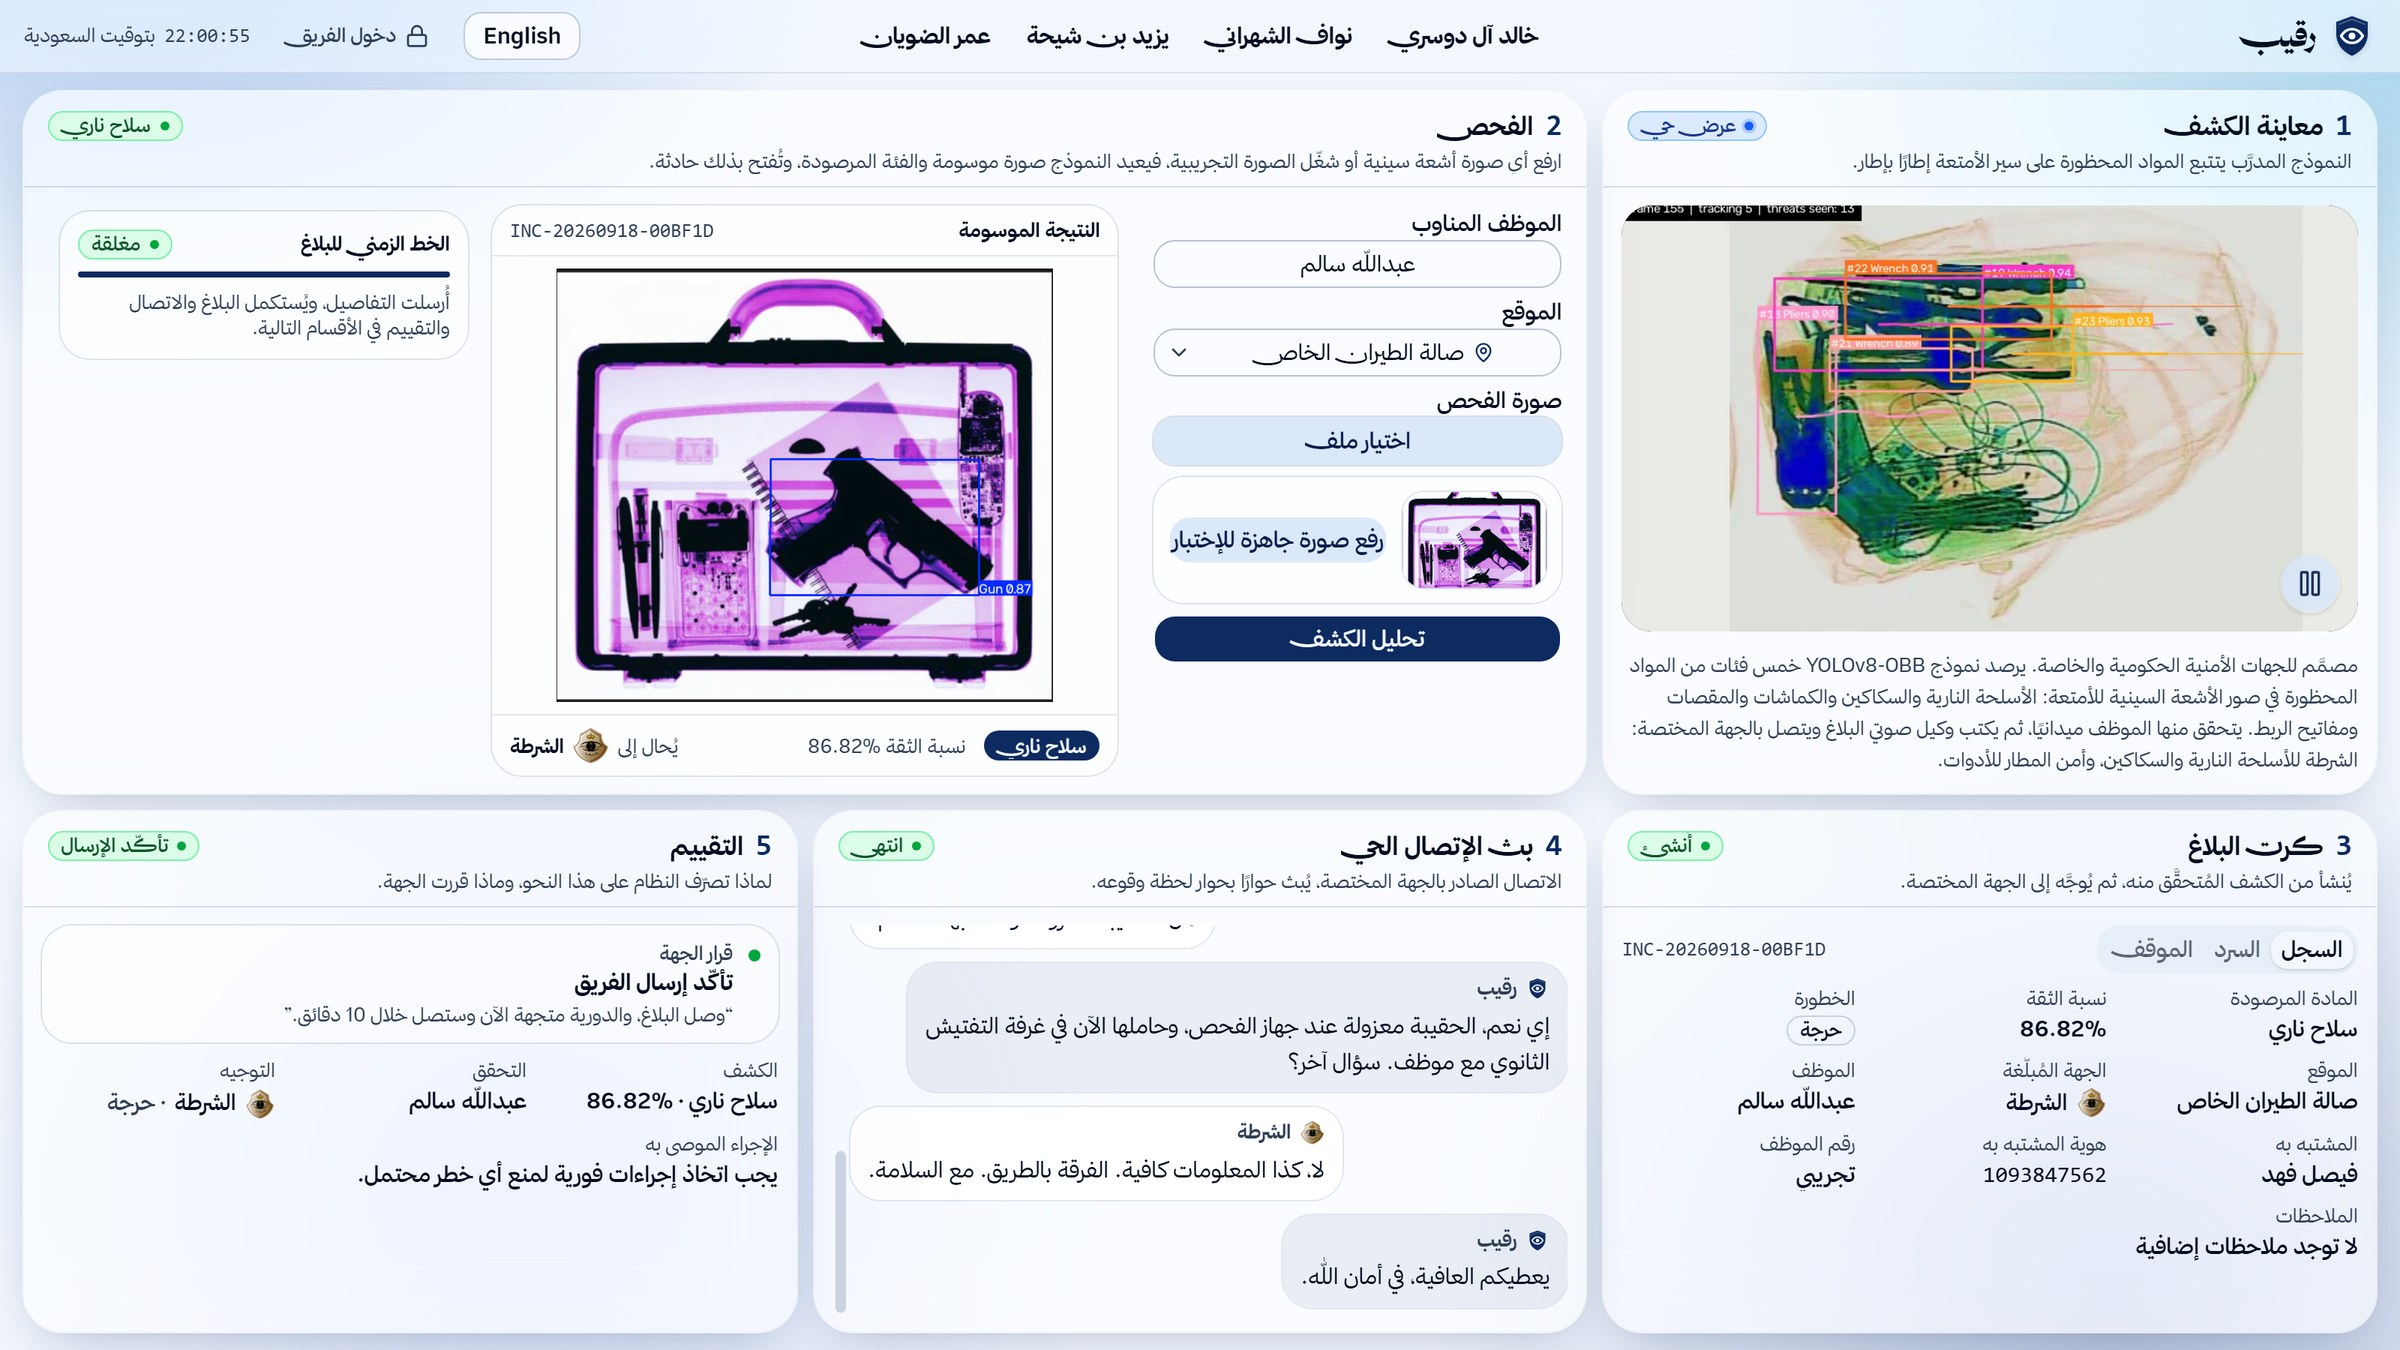
\includegraphics[width=\textwidth]{figures/ui_dashboard_arabic.jpg}
\caption{\textbf{The same incident in Arabic.} The interface is a full right-to-left layout, not only
translated labels.}
\end{figure}

\begin{figure}[H]
\centering
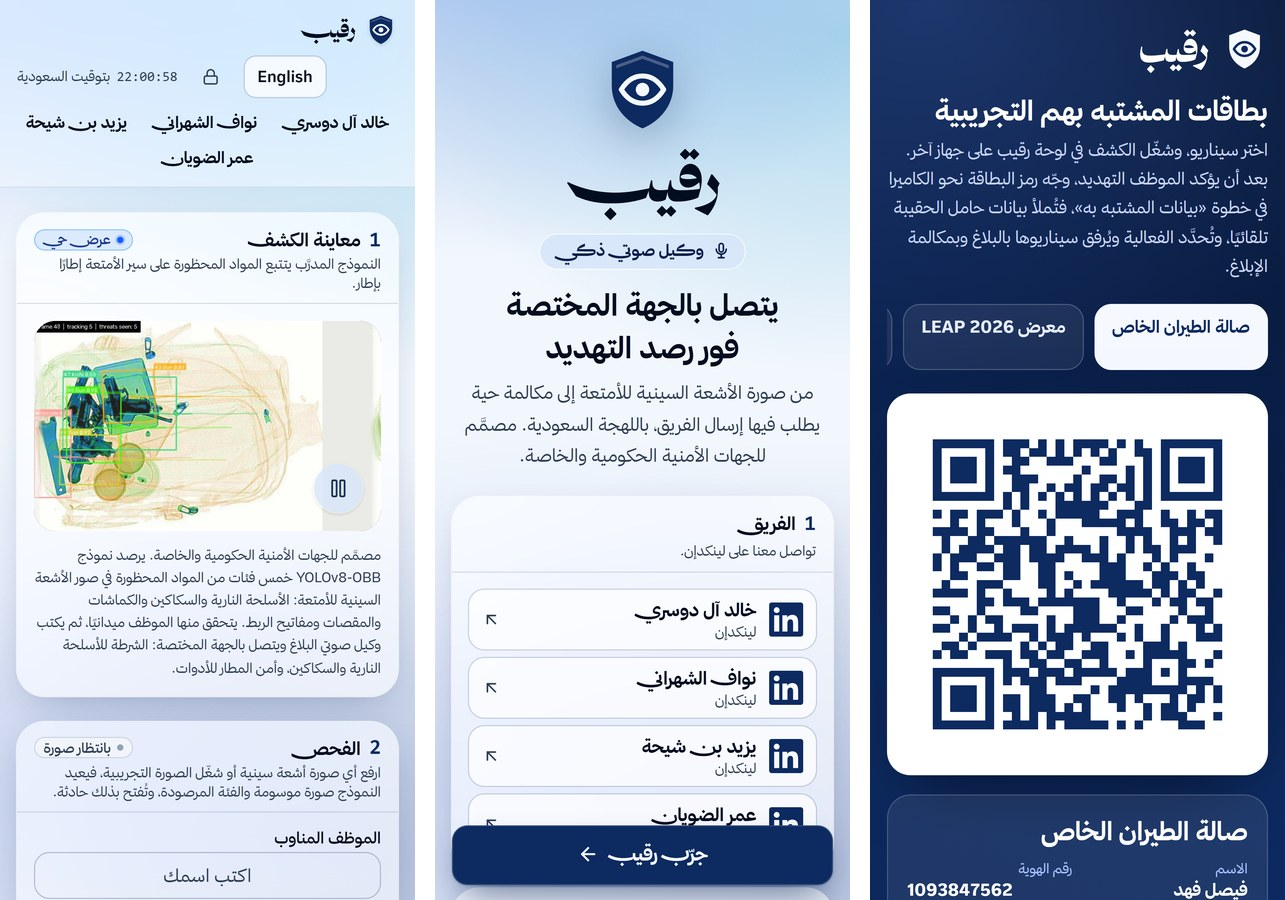
\includegraphics[width=0.92\textwidth]{figures/ui_phone_poster_passes.jpg}
\caption{\textbf{On a phone.} Left: the dashboard. Middle: the poster page
(\code{/poster}), opened from a printed poster's QR code. Right: the demo passes
(\code{/passes}), one per checkpoint, whose QR codes the dashboard can scan.}
\end{figure}

% ------------------------------------------------------------------ 7
\section{Results and evaluation}
\label{sec:results}

\subsection{Detection}

All numbers are measured on the 831 test images (1,593 objects) that were never used in training.
They were re-run for this report from the committed weights, and match \code{Model\_Training.ipynb}.

\begin{table}[H]
\centering
\small
\begin{tabular}{@{}lrrrrr@{}}
\toprule
Model & Precision & Recall & F1 & mAP50 & mAP50-95 \\
\midrule
Baseline (pretrained, not fine-tuned) & 0.028 & 0.030 & 0.029 & 0.004 & 0.002 \\
Experiment 1: yolov8n-obb & 0.947 & 0.856 & 0.899 & 0.900 & 0.765 \\
\textbf{Experiment 2: yolov8s-obb (final)} & \textbf{0.948} & \textbf{0.891} & \textbf{0.919} & \textbf{0.919} & \textbf{0.806} \\
\bottomrule
\end{tabular}
\caption{Test-set results. F1 is computed from the precision and recall that Ultralytics reports.}
\label{tab:results}
\end{table}

\textbf{What the metrics mean.} Precision is the share of detections that are real items; recall is
the share of real items that are found; mAP50 averages precision over all confidence thresholds when
a box counts as correct at 50\% overlap, and mAP50-95 repeats this at stricter overlaps, so it also
rewards precise boxes. For a screening aid, \textbf{recall matters most}: a missed gun is worse than a
false alarm, which the officer clears by hand in seconds.

\textbf{Why experiment 2 was chosen.} The larger model raised recall from 0.856 to 0.891 at the same
precision, and mAP50-95 from 0.765 to 0.806. It is about three times slower (58 ms against 21 ms per
image on a CPU), which is still fast enough for one image per bag.

\begin{table}[H]
\centering
\small
\begin{tabular}{@{}lrrrrrrr@{}}
\toprule
Class & Test objects & Precision & Recall & F1 & mAP50 & mAP50-95 & Missed at conf. 0.25 \\
\midrule
Gun      & 474 & 0.983 & 0.970 & 0.977 & 0.975 & 0.881 & 14 (3\%) \\
Knife    & 169 & 0.953 & 0.805 & 0.873 & 0.837 & 0.705 & 36 (21\%) \\
Pliers   & 524 & 0.941 & 0.891 & 0.916 & 0.909 & 0.804 & 59 (11\%) \\
Scissors & 120 & 0.956 & 0.905 & 0.930 & 0.948 & 0.845 & 11 (9\%) \\
Wrench   & 306 & 0.908 & 0.886 & 0.897 & 0.924 & 0.793 & 34 (11\%) \\
\bottomrule
\end{tabular}
\caption{Final model, per class. The last column counts objects with no correct detection at the
app's threshold (confidence 0.25, overlap 0.5).}
\label{tab:perclass}
\end{table}

\textbf{Errors at the app's threshold.} Matching every prediction to the labels at confidence 0.25,
the model finds 1,439 of the 1,593 objects (90\%). It misses 154, gives the wrong class 18 times, and
makes 94 detections that match no labelled object. 667 of the 831 images (80\%) are completely
right: every object found and nothing extra.

\begin{figure}[H]
\centering
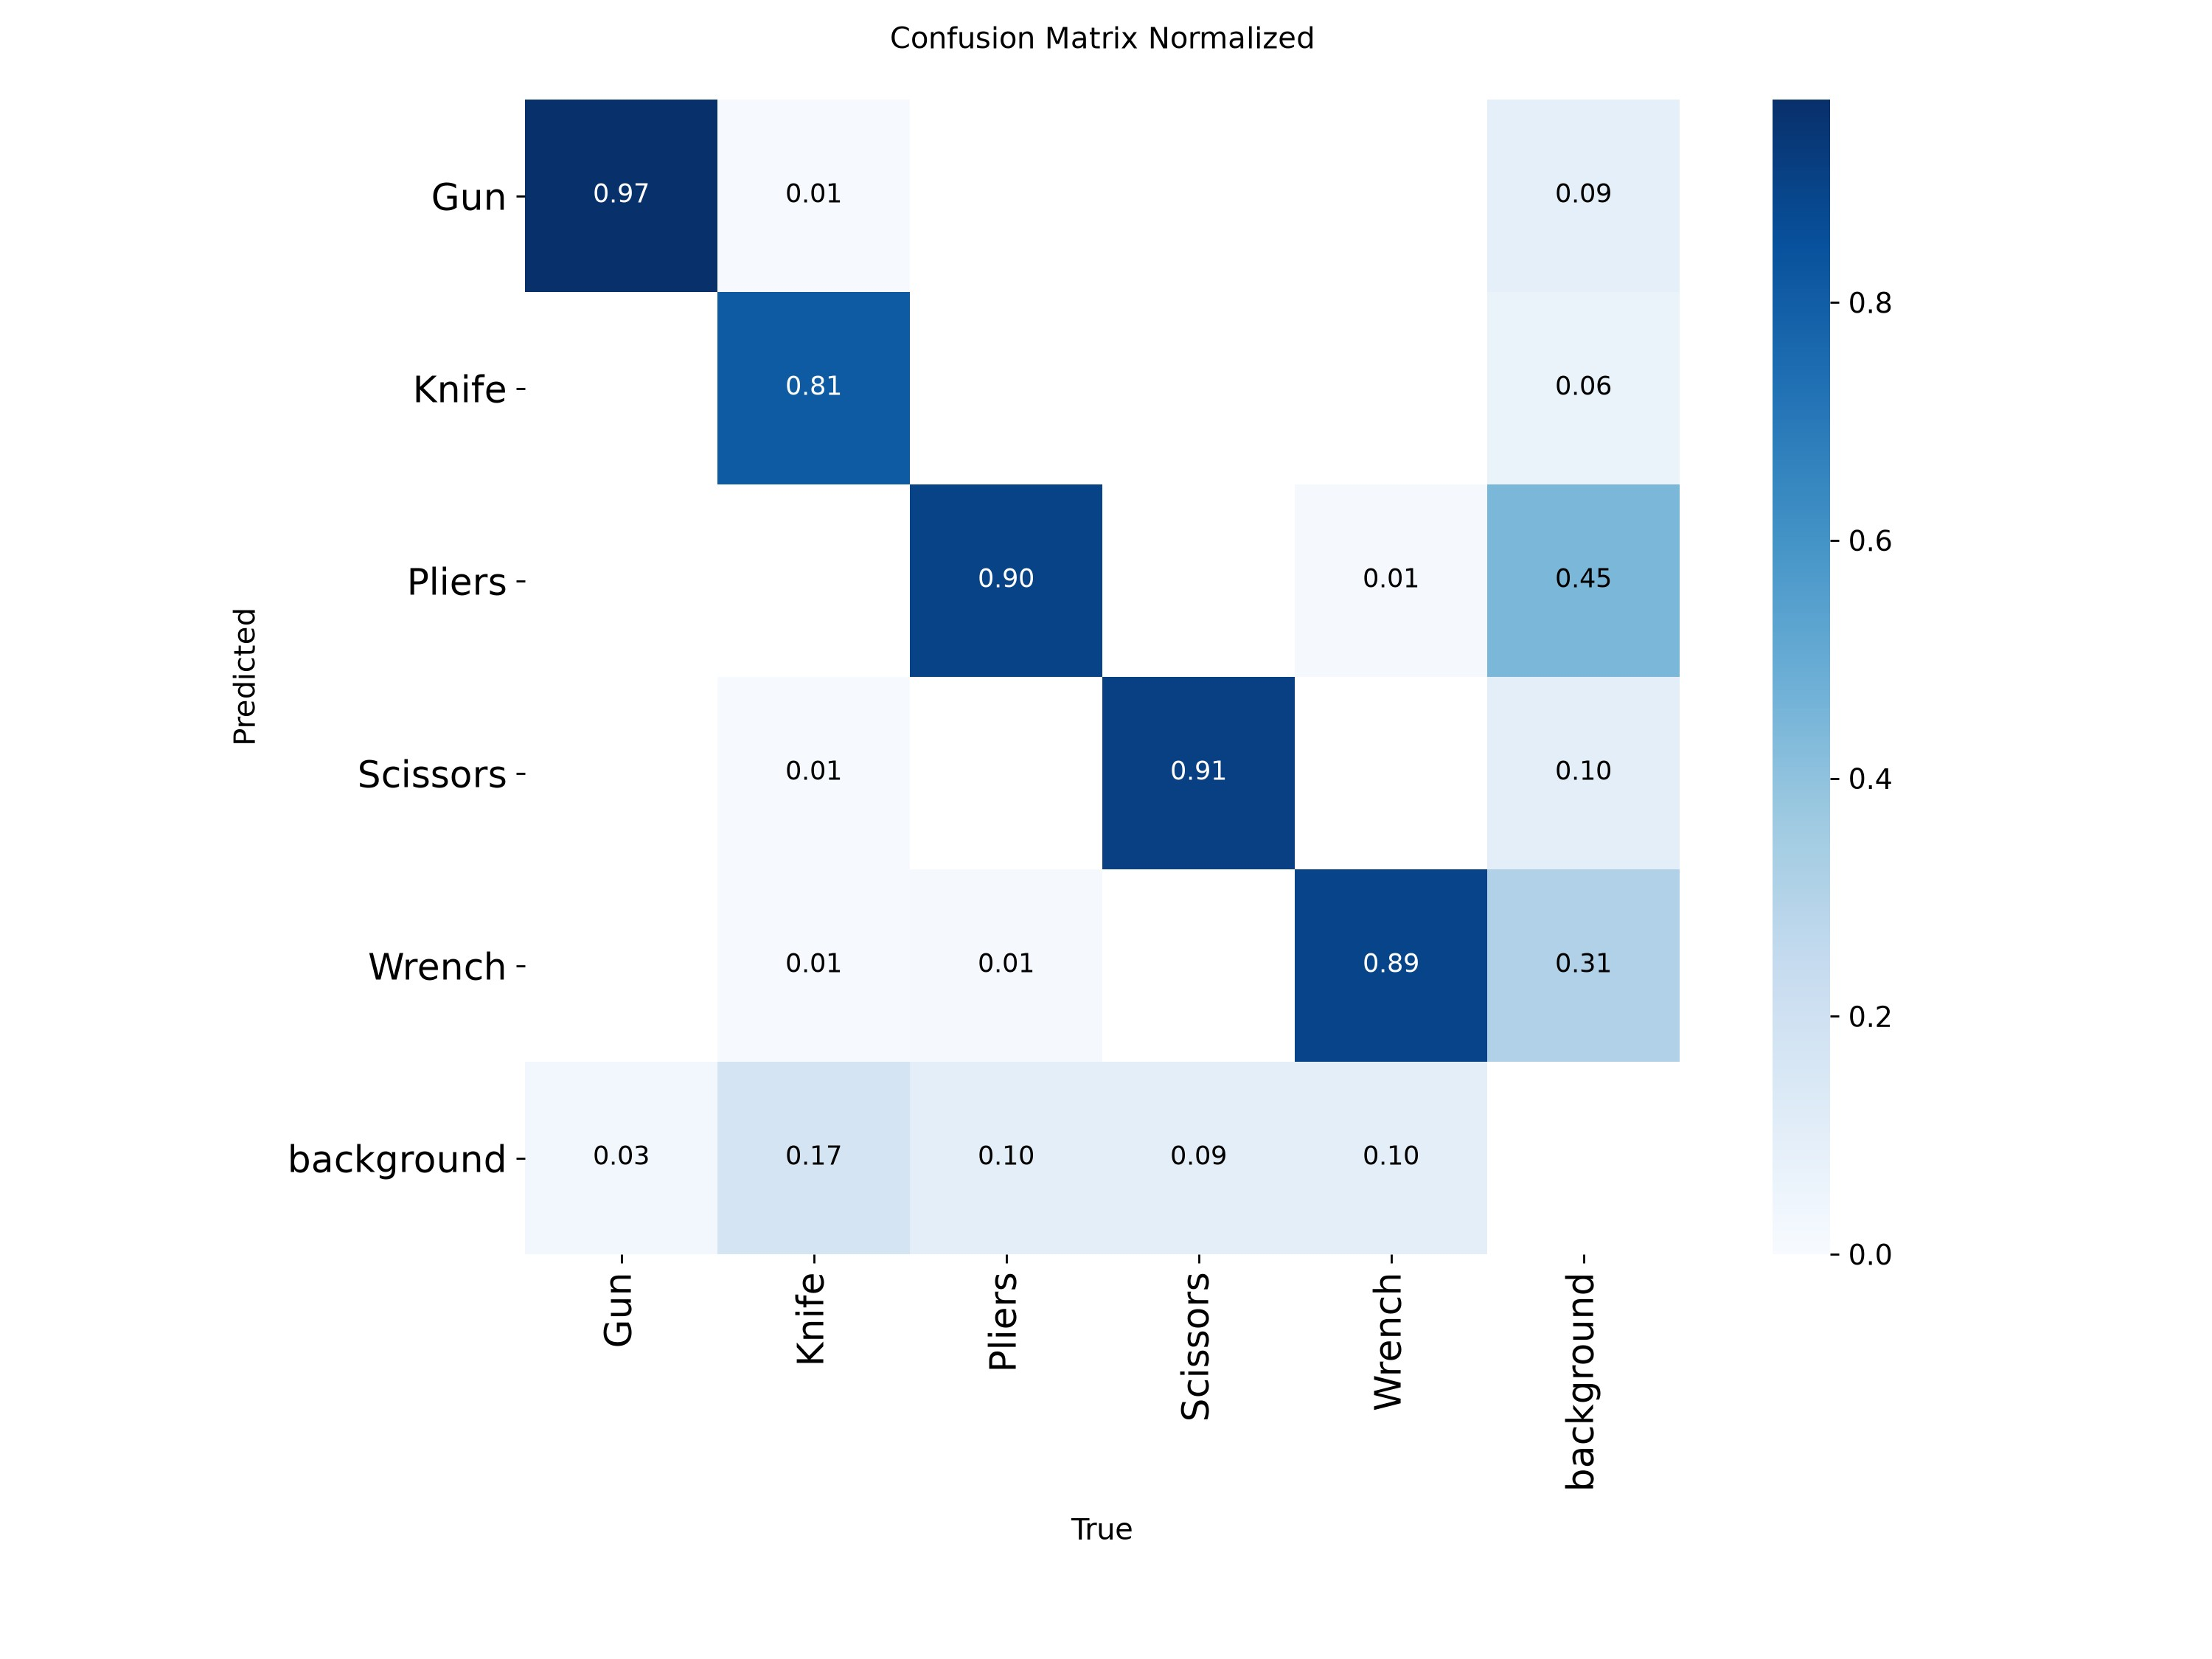
\includegraphics[width=0.74\textwidth]{figures/confusion_matrix.jpg}
\caption{Normalised confusion matrix of the final model on the test set (columns: true class). The
model almost never mistakes one item for another; every off-diagonal cell between classes is 0.01 or
less. Its errors are misses (bottom row: 17\% of knives) and extra detections (right column: mostly
pliers and wrenches).}
\label{fig:confusion}
\end{figure}

\begin{figure}[H]
\centering
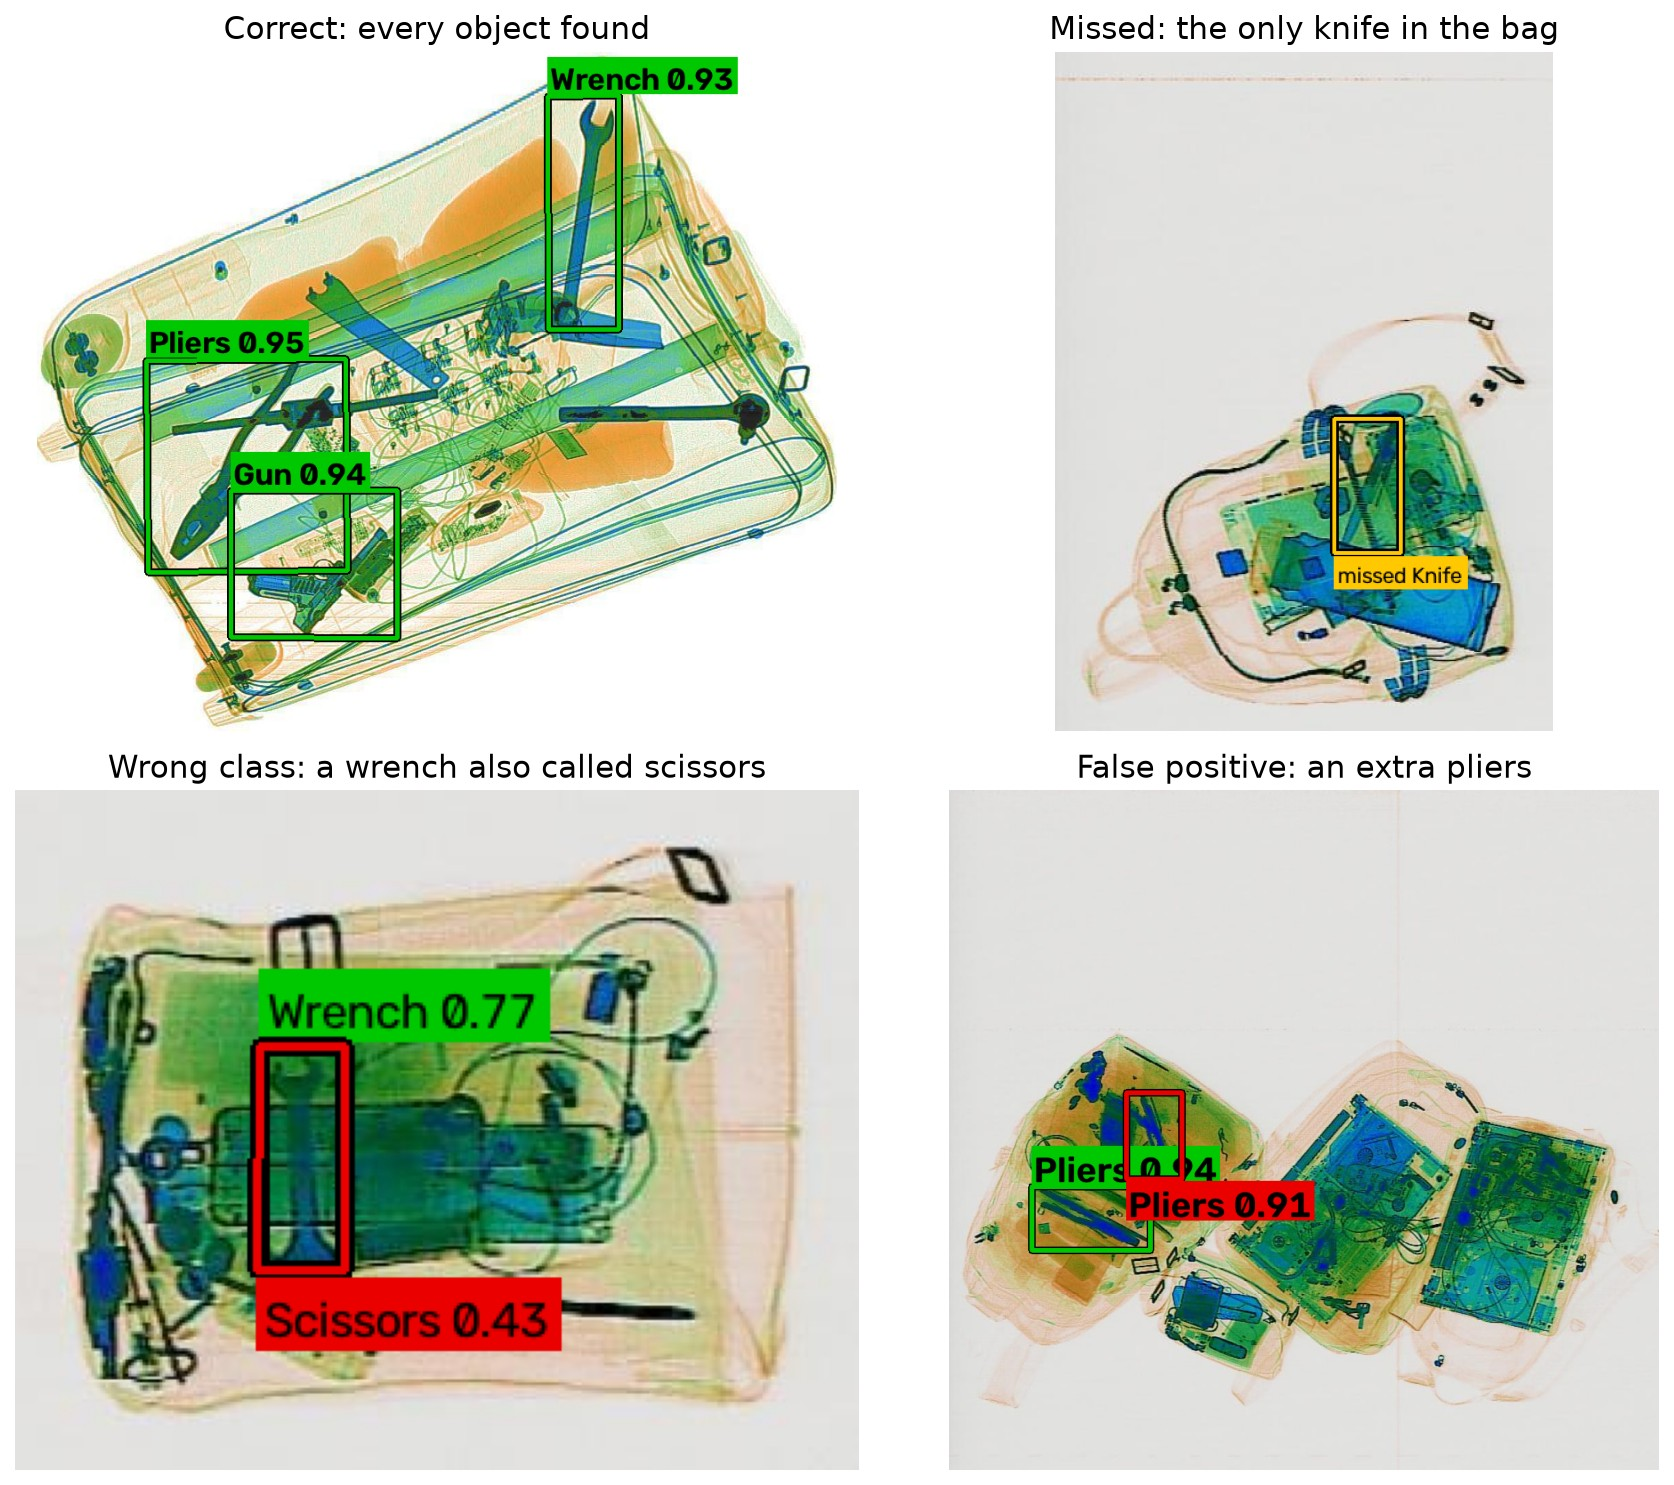
\includegraphics[width=0.86\textwidth]{figures/detection_examples.jpg}
\caption{Test images, final model. Green: correct detection. Orange: a labelled object the model
missed. Red: a wrong or extra detection. Top left: a bag where every item is found. Top right: a knife
that is the only object in the bag goes undetected. Bottom left: a wrench found correctly and also
labelled as scissors. Bottom right: an extra pliers detection on an unlabelled object.}
\label{fig:examples}
\end{figure}

\textbf{Interpretation.}
\begin{itemize}
  \item \textbf{Guns are the strongest class} (recall 0.97): they are the most distinctive shape and
        the second most common class.
  \item \textbf{Knives are the weakest}: one in five is missed. They have the second fewest examples,
        and a thin blade seen edge-on is a narrow line in the image, easily lost among cables and
        frames, as in figure~\ref{fig:examples}.
  \item \textbf{Most false alarms are pliers and wrenches}, the tool-like classes. Some of these may
        be real tools the annotators did not label, so the false-alarm count is an upper bound.
  \item \textbf{For the product this means} the model is a strong second pair of eyes, but it cannot
        replace the officer: the officer's own check stays in the workflow, and knives need the most
        attention.
\end{itemize}

\subsection{Tracking on video}
\label{sec:tracking}

On the synthetic belt clips (section 3.3), \code{track\_video.py --gt} scores tracking with the
standard CLEAR-MOT metrics~\cite{clearmot} and IDF1~\cite{idf1}. The key finding was a bug in how
video was fed to the model, not a weakness of the model: at the training size of 640 px, the
960 × 580 belt frames are shrunk so far that thin objects vanish.

\begin{table}[H]
\centering
\small
\begin{tabular}{@{}lrrrr@{}}
\toprule
Inference size & Wrench recall & Scissors recall & Pliers recall & Speed (CPU) \\
\midrule
640 px  & 0.016 & 0.038 & 0.695 & 20.9 fps \\
960 px  & 0.543 & 0.453 & 0.761 & 11.0 fps \\
\textbf{1280 px} & \textbf{0.814} & \textbf{0.604} & 0.746 & 6.4 fps \\
\bottomrule
\end{tabular}\hspace{0.6cm}
\begin{tabular}{@{}lrr@{}}
\toprule
Seed 21 & 640 px & 1280 px \\
\midrule
MOTA & 0.659 & \textbf{0.786} \\
IDF1 & 0.801 & \textbf{0.865} \\
Missed boxes & 567 & \textbf{346} \\
False positives & 143 & \textbf{97} \\
Mostly tracked & 21/30 & \textbf{26/30} \\
\bottomrule
\end{tabular}
\caption{Left: recall on belt video by inference size. Right: tracking on one clip. Misses and false
positives both fell, so the larger size was pure gain, and it is now the default for video.}
\end{table}

\begin{figure}[H]
\centering
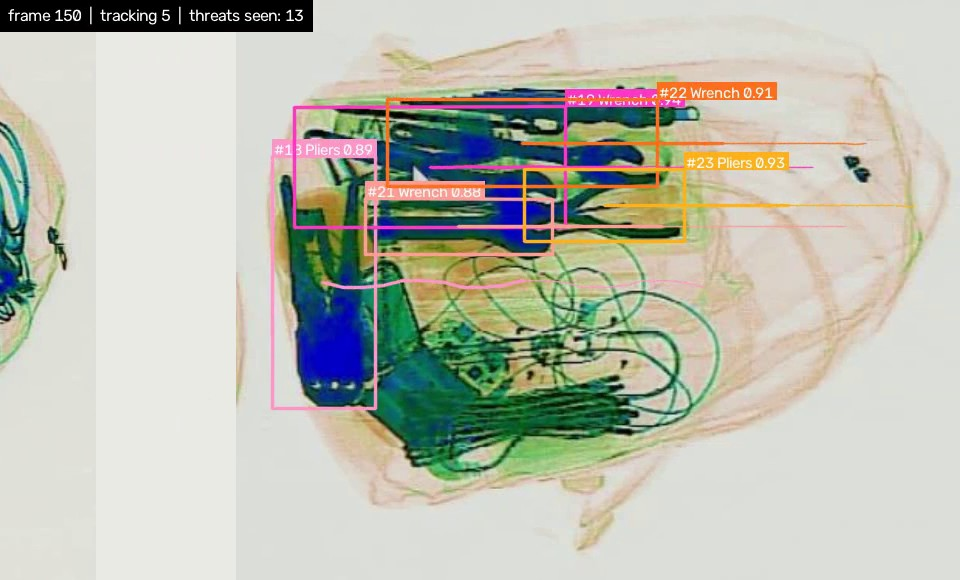
\includegraphics[width=0.62\textwidth]{figures/tracking_frame.jpg}
\caption{A frame of the dashboard's demo clip. Each item keeps its track ID (\#18, \#21, \ldots) and
leaves a motion trail; the counter at the top reports distinct threats rather than detections.}
\end{figure}

Two more findings: occlusion was not the problem (recall where bags overlap was 0.971, higher than
0.731 without overlap), and while identities hold well (IDF1 0.87), the number of distinct items is
still off by a few per clip, which only a better detector can fix.

\subsection{Language model}
\label{sec:llm}

\code{Report\_generation.ipynb} runs both prompts on the same five cases, built from real detections on
repository images, and checks every report automatically and by reading it.

\begin{table}[H]
\centering
\small
\begin{tabular}{@{}lcc@{}}
\toprule
In five reports & Prompt v1 (prototype) & Prompt v2 (production) \\
\midrule
Item named correctly & 5 & 5 \\
Detector confidence stated & 0 (never given it) & 5 \\
Placeholders left, such as ``[Your Name]'' & 5 & 0 \\
Invented actions & 5 & 1 \\
Names changed & 0 & 1 \\
Language & English & Arabic \\
Seconds per report & 3 to 6 (one call) & 8 to 11 (two calls) \\
\bottomrule
\end{tabular}
\caption{Prompt comparison, from the run saved in the notebook.}
\end{table}

\begin{itemize}
  \item \textbf{v1} invented what staff had done in every report (``the individual has been detained
        and is awaiting the arrival of the Armed Response Unit''), put tools in the airport's lost and
        found, called event venues airports, and left the author as a placeholder.
  \item \textbf{v2} kept the facts that decide the response: the item, the confidence, the suspect's
        ID number and the checkpoint. It stated missing information instead of inventing it, and set
        sensible severities: critical for the gun, high for the knife and medium for the tools. For
        pliers the detector was unsure of, the report says the confidence is not high.
  \item \textbf{v2 is not flawless.} Reading the Arabic turned up an invented investigation
        (\ar{فتح تحقيق فوري}), a claim that the way the gun was packed shows an intent to use it, a
        wrench called a lever, and a changed suspect name. Earlier runs invented an arrest and
        recommended searching for a screwdriver when the item was a wrench. This is why the record
        sent to the authority and the call's briefing use the structured fields, never the model's
        prose.
\end{itemize}

\subsection{The complete system}

\begin{itemize}
  \item \textbf{Automated tests:} 40 tests pass, driving the whole workflow with mock providers: the
        false-alarm branch, validation of the carrier's details, routing, calls that reach no one,
        the Arabic-only call instructions, and the public and signed-in modes.
  \item \textbf{A full run} (the screenshots in section 6): detection to finished report in about 20
        seconds, and a call of about two and a half minutes that ended with the dispatch confirmed and the
        authority's words recorded.
  \item \textbf{Failure handling was also observed:} in one attempt the network failed while the call
        was being set up, and the incident was held as ``call unanswered'' with a ``Call again''
        button, as designed, instead of being lost.
\end{itemize}

% ------------------------------------------------------------------ 8
\section{Challenges and limitations}

\subsection{Challenges}

\begin{itemize}
  \item \textbf{No X-ray video exists publicly.} We generated belt footage with known identities from
        the test images so tracking could be measured instead of judged by eye.
  \item \textbf{Small and thin objects.} Knives and wrenches are easily lost; the inference-size
        finding in section~\ref{sec:tracking} recovered most of that on video.
  \item \textbf{Imbalanced classes.} Handled by oversampling (section 3.2); knives remain the weakest
        class.
  \item \textbf{No local GPU.} Training ran on rented A100s through Modal, for about US\$4 to 5 in total.
  \item \textbf{Language-model errors.} The first prompt invented facts freely; the second still does
        occasionally (section~\ref{sec:llm}).
  \item \textbf{Telephony.} Calls to Saudi numbers were refused until Twilio's geographic permissions
        were set; one call reached voicemail and was once recorded as a confirmation, which led to the
        rule that no decision is recorded before the other side speaks; the provider's answering-machine
        detection judged real people to be machines three times in five and was removed; and phones
        that silence unknown callers never ring.
  \item \textbf{Deployment.} The backend scales to zero, so the first request after a quiet period
        takes about ten seconds, and paused incidents had to move from memory to a database to survive
        a container change.
\end{itemize}

\subsection{Limitations}

\begin{itemize}
  \item \textbf{Five classes only.} Explosives, liquids and every other threat are invisible to the
        model.
  \item \textbf{One dataset, one kind of scanner.} Accuracy on other scanners' images is unknown.
  \item \textbf{One item per report.} The report is written about the most confident detection in an
        image; a bag with several different items is reported by its strongest one. The officer
        sees every box, but the report does not.
  \item \textbf{Occasional errors in the Arabic report} and in the live transcription of the other side:
        in one call the phrase \ar{الفرقة بالطريق} (the team is on its way) was transcribed as a
        non-word.
  \item \textbf{Synthetic tests.} The tracking numbers come from generated video, and the call in
        section 6 used a recorded reply rather than a real officer.
\end{itemize}

\subsection{Future improvements}

\begin{itemize}
  \item Train at a larger image size and with more knife examples, to raise knife recall.
  \item Pass every confirmed box to the report, not just the most confident one.
  \item Choose the recommended action from a fixed list per class, and lower the report's
        temperature, to remove the remaining invented details.
  \item Test with real officers and real scanner images before any operational use.
\end{itemize}

\subsection{Responsible use and privacy}

\begin{itemize}
  \item Raqeeb supports a decision; it does not make one. A person checks every bag before anything is
        reported, and the officer can reject any detection.
  \item All people, passes and scenarios in the demo are fictional; no real personal data was used.
        The team's own phone numbers live only in server configuration, not in the code or the
        dashboard.
  \item The public demo cannot phone anyone, and each public conversation is limited to one per
        incident and three minutes.
  \item The police emblem comes from Wikimedia Commons under CC BY-SA 4.0 and is credited in the
        repository, in \path{frontend/public/authorities/CREDITS.md}. The licence also asks for a visible credit on the
        site, which is still to be added.
\end{itemize}

% ------------------------------------------------------------------ 9
\section{Team contributions}
\label{sec:team}

\begin{table}[H]
\centering
\small
\begin{tabularx}{\textwidth}{@{}P{3.6cm}L@{}}
\toprule
Member & Contribution \\
\midrule
Khalid Al Dosari & Data analysis and preprocessing (\code{EDA.ipynb}); training and evaluating both
detectors on Modal (\code{Model\_Training.ipynb}, \code{modal\_train.py}); the React dashboard,
passes and poster pages; deployment (Modal, Vercel,
Cloudflare); hardening the call flow (Arabic call, live transcript, unanswered calls, public and
signed-in modes); the prompt evaluation notebook and this report \\
Nawaf Alsharani & The report generator: the first report-generation prototype and its prompt (prompt v1
in section~\ref{sec:llm}) \\
Yazeed Bin Shihah & The voice agent application: the LangGraph incident workflow, the FastAPI routes,
the provider interfaces and Twilio integration, and the OpenAI realtime provider with SIP bridging \\
Omar Al-Dhawyan & The tracking mechanism: following each item across video frames with a tuned
BoT-SORT tracker (\code{track\_video.py}); and the video generation: synthetic belt footage with
ground truth, used to measure tracking (\code{make\_test\_video.py}) \\
\bottomrule
\end{tabularx}
\caption{Who did what.}
\end{table}

% ------------------------------------------------------------------ 10
\section{Links}

\begin{table}[H]
\centering
\small
\begin{tabularx}{\textwidth}{@{}P{3.8cm}L@{}}
\toprule
GitHub repository & \url{https://github.com/khaliddosari/Raqeeb} \\
Live demo & \url{https://raqeeb.khalid-ai.dev} \\
Poster page & \url{https://raqeeb.khalid-ai.dev/poster} \\
Demo passes & \url{https://raqeeb.khalid-ai.dev/passes} \\
Dataset & \href{https://universe.roboflow.com/khalid-abdullah-al-dosari/sixray-gzyn7}{\nolinkurl{universe.roboflow.com/khalid-abdullah-al-dosari/sixray-gzyn7}} \\
Original benchmark & \url{https://github.com/MeioJane/SIXray} \\
Detector & YOLOv8-OBB, \url{https://docs.ultralytics.com/tasks/obb/}; trained weights
\code{best\_yolov8s.pt} in the repository \\
Tracker & \url{https://docs.ultralytics.com/modes/track/} \\
Workflow & LangGraph, \url{https://langchain-ai.github.io/langgraph/} \\
Language and voice models & OpenAI \code{gpt-4o-mini} and \code{gpt-realtime}, through the OpenAI API \\
Hugging Face Space & None: the demo is hosted on Vercel and Modal \\
\bottomrule
\end{tabularx}
\end{table}

\begin{thebibliography}{9}
\footnotesize
\setlength{\itemsep}{0.1em}
\bibitem{sixray} C.~Miao, L.~Xie, F.~Wan, C.~Su, H.~Liu, J.~Jiao and Q.~Ye. SIXray: A large-scale
security inspection X-ray benchmark for prohibited item discovery in overlapping images. \emph{CVPR}, 2019.
\url{https://arxiv.org/abs/1901.00303}
\bibitem{yolov8} G.~Jocher, A.~Chaurasia and J.~Qiu. Ultralytics YOLOv8, 2023.
\url{https://github.com/ultralytics/ultralytics}
\bibitem{dota} G.-S.~Xia et al. DOTA: A large-scale dataset for object detection in aerial images.
\emph{CVPR}, 2018.
\bibitem{botsort} N.~Aharon, R.~Orfaig and B.-Z.~Bobrovsky. BoT-SORT: Robust associations
multi-pedestrian tracking. arXiv:2206.14651, 2022.
\bibitem{clearmot} K.~Bernardin and R.~Stiefelhagen. Evaluating multiple object tracking performance:
the CLEAR MOT metrics. \emph{EURASIP Journal on Image and Video Processing}, 2008.
\bibitem{idf1} E.~Ristani, F.~Solera, R.~Zou, R.~Cucchiara and C.~Tomasi. Performance measures and a
data set for multi-target, multi-camera tracking. \emph{ECCV Workshops}, 2016.
\end{thebibliography}

\end{document}
